\documentclass[t,aspectratio=169]{beamer}

\graphicspath{{img/}}

\usepackage{mathspec}

\usepackage{algorithm}
\usepackage{algpseudocode}
\usepackage[arrows]{boisik}
\usepackage{booktabs}
\usepackage[ngerman]{babel}
\usepackage{cancel}
\usepackage{changepage}
\usepackage{collect}
\usepackage{comment}
\usepackage{csquotes}
\usepackage{float}
\usepackage{graphbox}
\usepackage{hyperref}
\usepackage{listings}
\usepackage{multimedia}
\usepackage{tikz}
\usepackage[table]{xcolor}
\usepackage{siunitx}

% \setmainfont{Libertinus Serif}
% \setsansfont{Libertinus Sans}
% \setmonofont{TeX Gyre Cursor Bold}
% \setmathfont[Digits]{Libertinus Sans}

\setmainfont{Liberation Serif}
\setsansfont{Liberation Sans}
\setmonofont{Liberation Mono}
\setmathfont[Digits]{Liberation Sans}

\usetheme{Madrid}
\usecolortheme{spruce}
\setbeamercovered{invisible}
\setbeamercolor{alerted text}{fg=blue}

\setbeamertemplate{navigation symbols}{}

\usebeamercolor[bg]{palette primary}
\usebeamercolor[bg]{palette secondary}
\usebeamercolor[bg]{palette tertiary}


\newenvironment{itemblock}[1]{\begin{block}{#1}\begin{itemize}}{\end{itemize}\end{block}}
\newenvironment{withtitle}[1]{\begin{description}\item[#1]~\\}{\end{description}}

\newcommand{\todo}[1]{\colorbox{red}{\color{white}\bf TODO: #1}}
\newcommand{\dunno}[0]{\colorbox{red}{\color{white}\bf ???}}

\newcommand{\uexplain}[2]{\underbrace{\mathtt{#1}}_{\hidewidth \mathsf{#2}\hidewidth} \hskip 0.5em}
\newcommand{\oexplain}[2]{\overbrace{\mathtt{#1}}^{\hidewidth \mathsf{#2}\hidewidth} \hskip 0.5em}

\definecollection{picture-sources}

\newcommand{\sourcedimage}[5][width=\textwidth,height=0.7\textheight,keepaspectratio]{%
  \begin{center}
    \includegraphics[#1]{#2}

    \expandafter\begin{collect}{picture-sources}{}{}
      \item[#3] \href{#4}{#4} \\ #5
    \end{collect}
  \end{center}
}

\newcommand{\imageframe}[4]{%
  {
    \setbeamercolor{background canvas}{bg=black}
    \begin{frame}[c,plain]
        \expandafter\begin{collect}{picture-sources}{}{}
        \item[#2] \href{#3}{#3} \\ #4
        \end{collect}
        \begin{tikzpicture}[remember picture,overlay]
          \node[at=(current page.center)] {
            \includegraphics[width=\paperwidth,height=\paperheight,keepaspectratio]{#1}
          };
        \end{tikzpicture}
    \end{frame}
  }
}

\lstset{basicstyle=\ttfamily}

\renewcommand{\algorithmicforall}{\textbf{for each}}

\title[~]{\Huge Computer selbst bauen}
\subtitle{}
\author[~]{andi $\langle$andi@entropia.de$\rangle$}
\date{}

\begin{document}

{
  \setbeamercolor{background canvas}{bg=black}
  \begin{frame}[plain]
    \begin{tikzpicture}[remember picture,overlay]
      \node[at=(current page.center)] {
        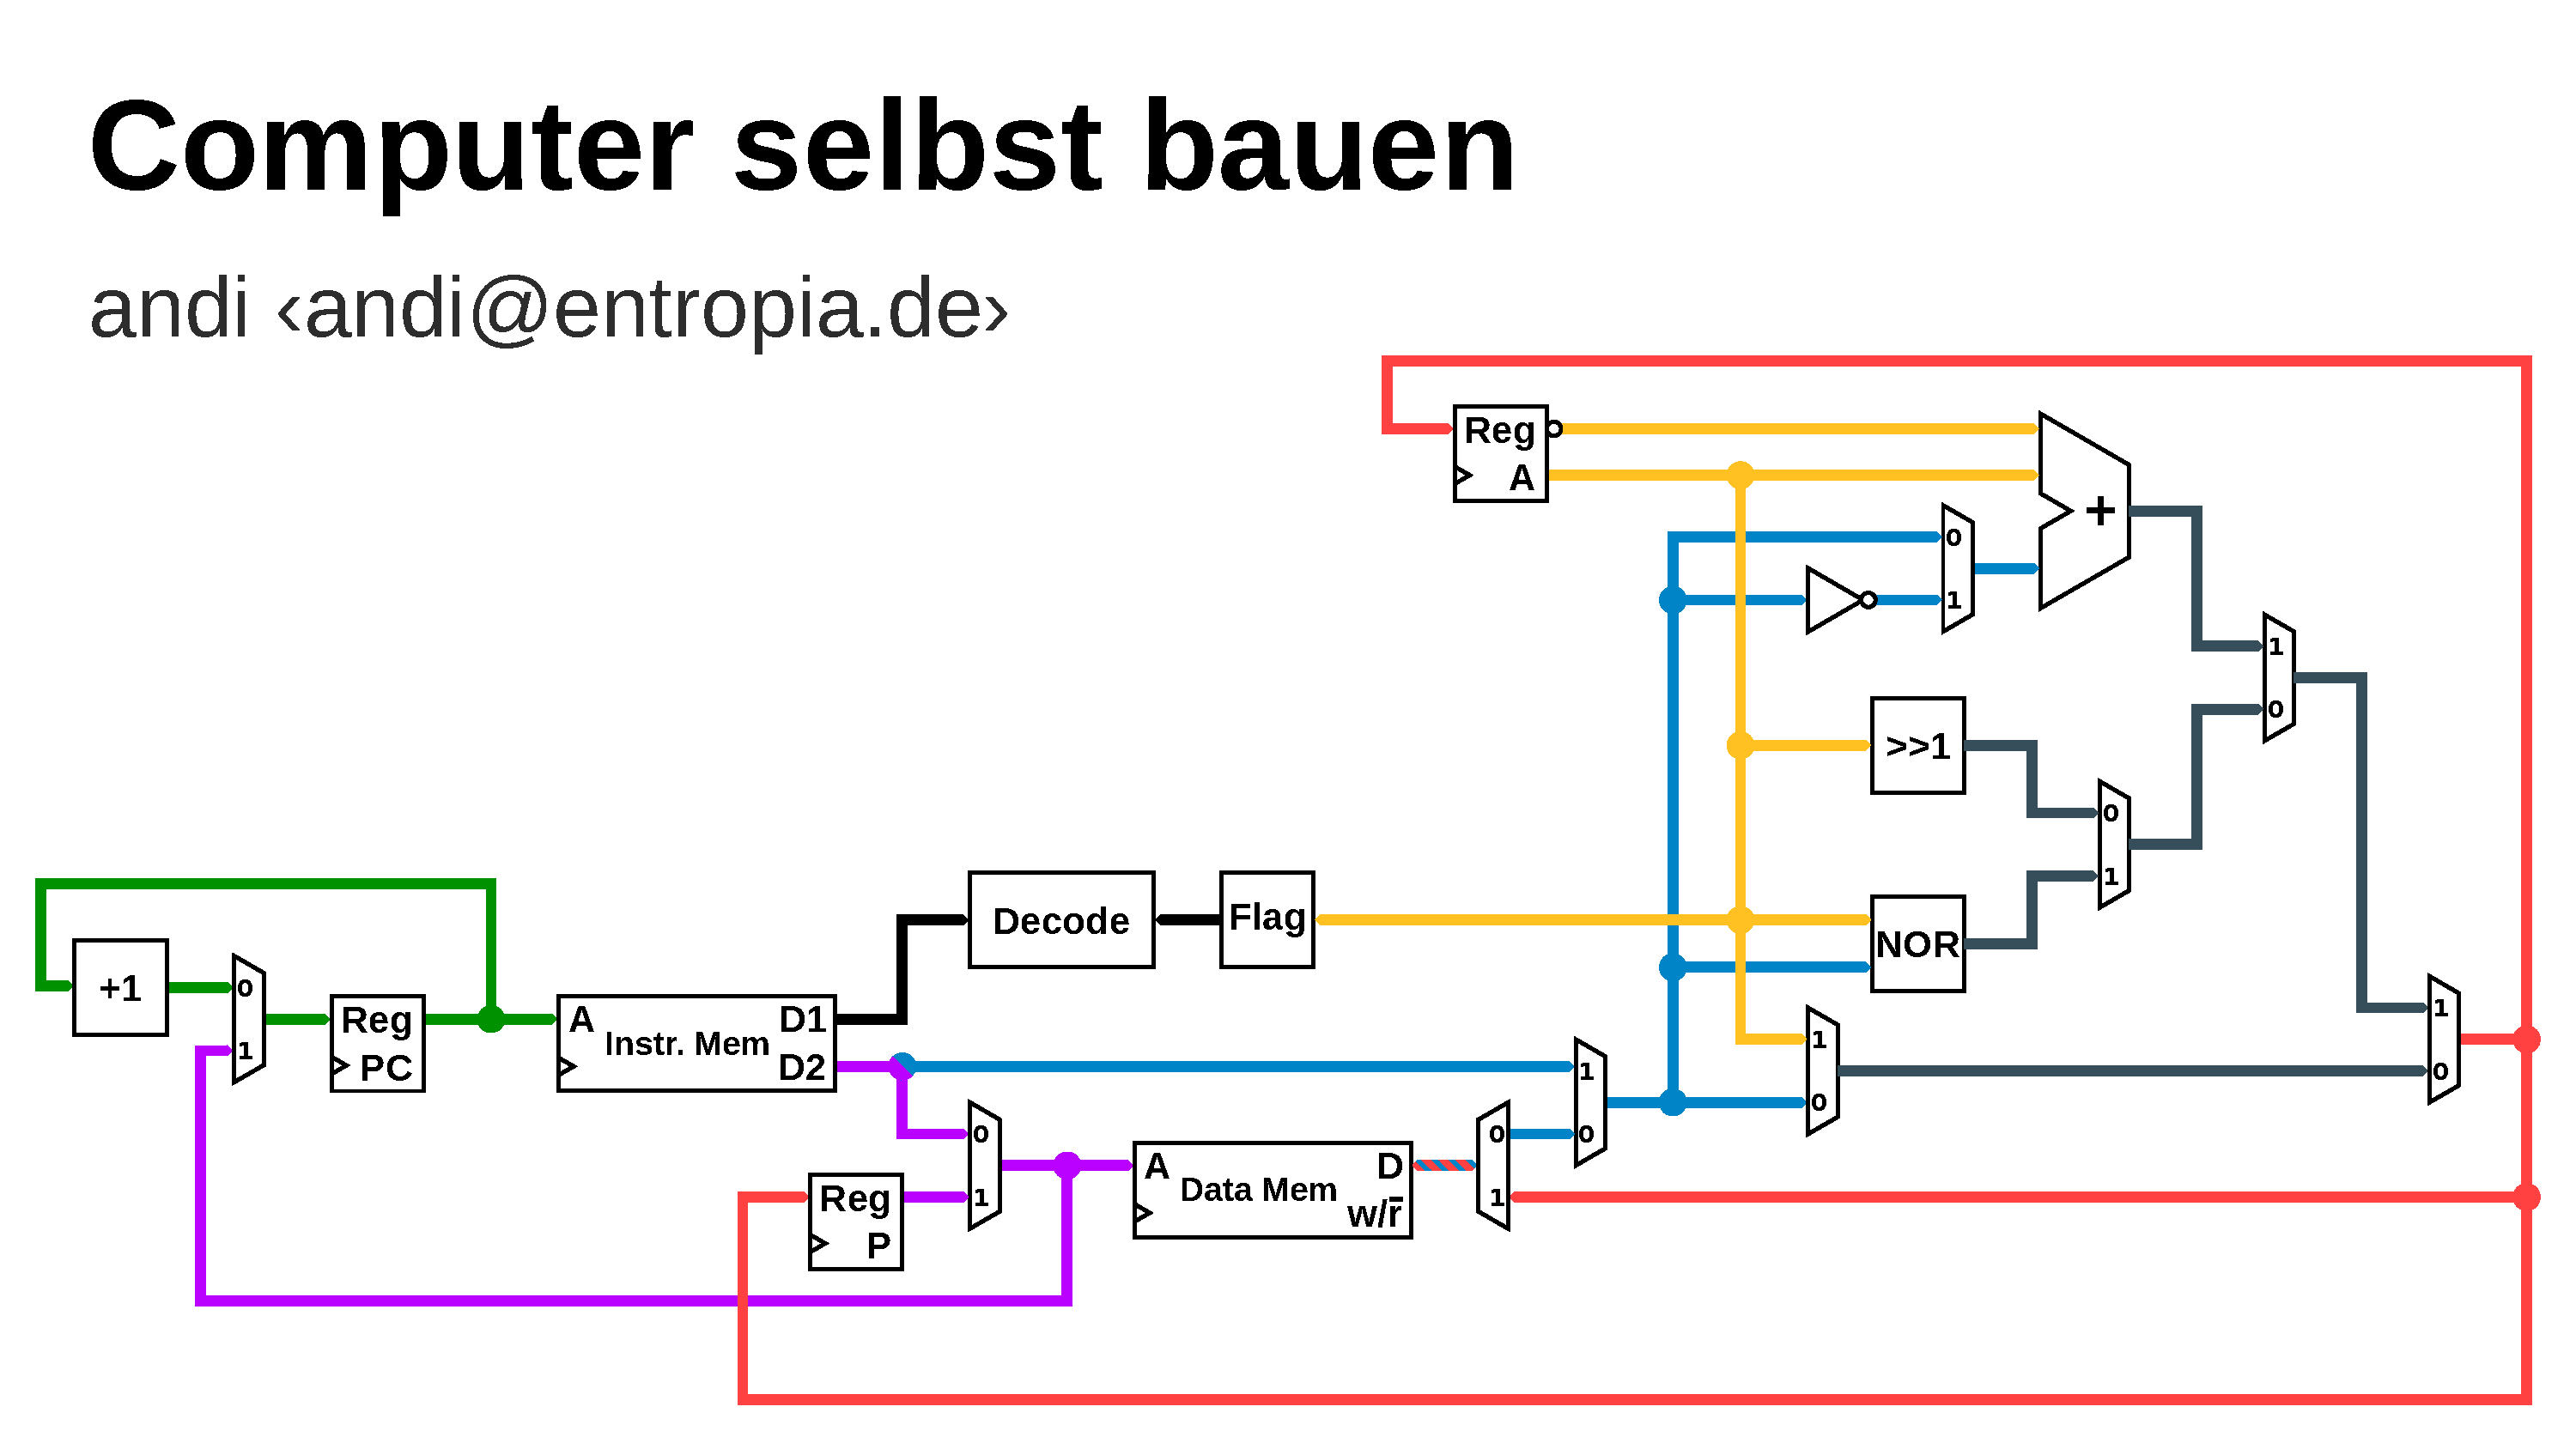
\includegraphics[width=\paperwidth,height=\paperheight,keepaspectratio]{title-slide}
      };
    \end{tikzpicture}
  \end{frame}
}

\begin{frame}
  \frametitle{Es ist kompliziert}

  \begin{columns}
    \begin{column}{.45\textwidth}
      \begin{center}
        \sourcedimage{zen2-die-shot}{Die Shot eines AMD Zen2}{https://en.wikipedia.org/wiki/File:Zen2\_Matisse\_Ryzen\_7nm\_Core\_Die\_shot.jpg}{Fritzchens Fritz, 2019. CC-0.}
        \emph{AMD Zen 2 \enquote{Matisse}}
      \end{center}
    \end{column}
    \begin{column}{.45\textwidth}
      \begin{itemize}
      \item \qty{4800000000} Transistoren
      \item Taktzeit:\\
        \qty{0.2}{\nano\second} $\hat=$ \qty{6.4} Licht-cm $\approx$ \qty{4} Strom-cm
      \end{itemize}

      \bigskip

      Mehr dazu:

      \smallskip

      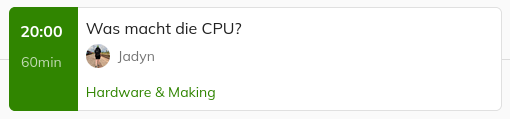
\includegraphics[width=\textwidth]{talk-jadyn}
    \end{column}
  \end{columns}
\end{frame}

\begin{frame}
  \frametitle{Es geht einfacher}

  \begin{columns}
    \begin{column}{.45\textwidth}
      \sourcedimage{relay-transparent}{Transparentes Relais}{https://commons.wikimedia.org/wiki/File:Omron\_G2R-2-24V\_relay\_04.jpg}{Retired electrician, 2022. CC-0.}
    \end{column}
    \begin{column}{.45\textwidth}
      \begin{itemize}
      \item \qty{120} Relais
      \item Takt: $\approx$ \qty{1}{\second}
      \end{itemize}
    \end{column}
  \end{columns}
\end{frame}

\begin{frame}
  \frametitle{0, 1, Logik}

  \begin{center}
    MOSFET, BJT, Röhren, Ringkerne, Opamps, Relais, Hydraulik, Lochbleche, \ldots

    \textit{Alles das Gleiche und sowieso nur Gefrickel!}
  \end{center}

  \begin{columns}[t]
    \begin{column}{.45\textwidth}
      \begin{block}{Signale}
        \begin{itemize}
        \item binärer Rechner $\Rightarrow$ 0 und 1\\
          \uncover<2->{\ldots{} und Z} \uncover<3->{\ldots{} und L und H \ldots}
        \item Signalübertragung (also Kabel \ldots)
        \end{itemize}
      \end{block}
    \end{column}
    \begin{column}{.45\textwidth}
      \begin{block}{Gates}
        Beliebige Gates sind erlaubt, spezifiziert durch \enquote{kleine} I/O-Tabelle

        \begin{center}
          \begin{tabular}{ccc}
            X & Y & out \\
            \midrule
            0 & 0 & 1 \\
            0 & 1 & 0 \\
            1 & 0 & 0 \\
            1 & 1 & 0 \\
          \end{tabular}
        \end{center}
      \end{block}
    \end{column}
  \end{columns}
\end{frame}

\begin{frame}
  \frametitle{Busse}

  \begin{columns}[T]
    \begin{column}{.45\textwidth}
      \begin{itemize}
      \item Signale gehören zusammen und tun \enquote{das Gleiche}
      \item übersichtlicher mit einer Linie\\
        (1 fette Linie $\hat=$ 8 dünne)\\
        und einem Gate
      \item nur (!) in unserem Kopf:\\
        Zahl, Adresse, Instruktion \ldots
      \end{itemize}
    \end{column}

    \begin{column}{.45\textwidth}
      \centering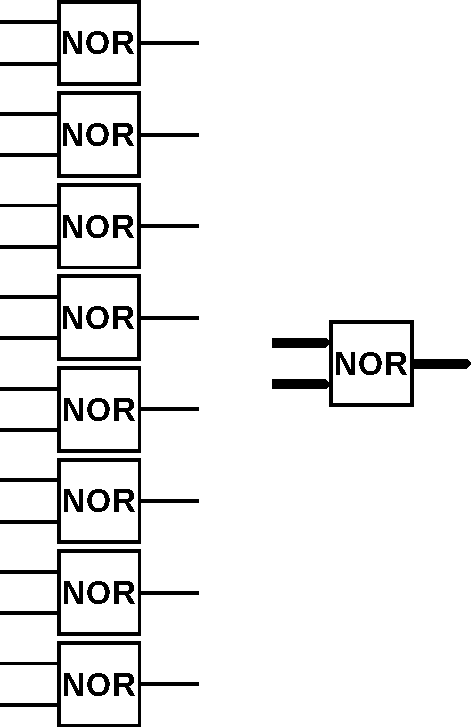
\includegraphics[height=.75\textheight]{nor-bus.pdf}
    \end{column}
  \end{columns}
\end{frame}

\begin{frame}
  \frametitle{Rechnen ist nicht schwer}

  \ldots zumindest Addieren:

  \begin{columns}
    \begin{column}{.45\textwidth}
      \begin{align*}
        0 + 0 + 0 = 00 \\
        0 + 0 + 1 = 01 \\
        0 + 1 + 0 = 01 \\
        1 + 0 + 0 = 01 \\
        1 + 1 + 0 = 10 \\
        \textcolor<2->{palette tertiary.bg}{1 + 0 + 1 = 10} \\
        0 + 1 + 1 = 10 \\
        1 + 1 + 1 = 11
      \end{align*}

      Auch nur ein Gate!
    \end{column}
    \begin{column}{.45\textwidth}
      \begin{center}
        \alt<2->{
          \begin{tabular}{ccccccccc}
            & 0 & 0 & 1 & 1 & \cellcolor{palette primary.bg}1 & 1 & 1 & 0 \\
            + & 0 & 0 & 0 & 1 & \cellcolor{palette primary.bg}0 & 1 & 0 & 1 \\
            &   &   & \scriptsize{1}  & \cellcolor{palette secondary.bg}\scriptsize{1}  & \cellcolor{palette primary.bg}\scriptsize{1}  &   &   &   \\
            \hline
            & 0 & 1 & 0 & 1 & \cellcolor{palette secondary.bg}0 & 0 & 1 & 1
          \end{tabular}
        }{
          \begin{tabular}{ccccccccc}
            & 0 & 0 & 1 & 1 & 1 & 1 & 1 & 0 \\
            + & 0 & 0 & 0 & 1 & 0 & 1 & 0 & 1 \\
            &   &   & \scriptsize{1}  & \scriptsize{1}  & \scriptsize{1}  &   &   &   \\
            \hline
            & 0 & 1 & 0 & 1 & 0 & 0 & 1 & 1
          \end{tabular}
        }

        \bigskip

        \uncover<3>{
          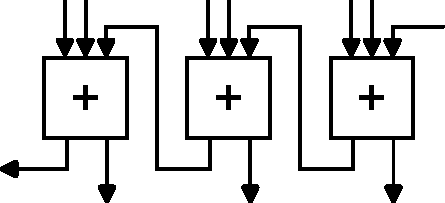
\includegraphics[width=.66\linewidth]{ripple-carry.pdf}
        }
      \end{center}
    \end{column}
  \end{columns}

\end{frame}

\begin{frame}
  \frametitle{Rechnen ist nicht schwer}

  \begin{center}
    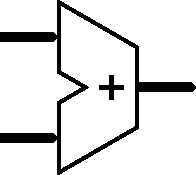
\includegraphics[height=.7\textheight]{adder.pdf}
  \end{center}
\end{frame}

\begin{frame}
  \frametitle{\ldots und fertig ist der \enquote{ASIC}}

  \begin{columns}
    \begin{column}{.45\textwidth}
      \begin{center}
        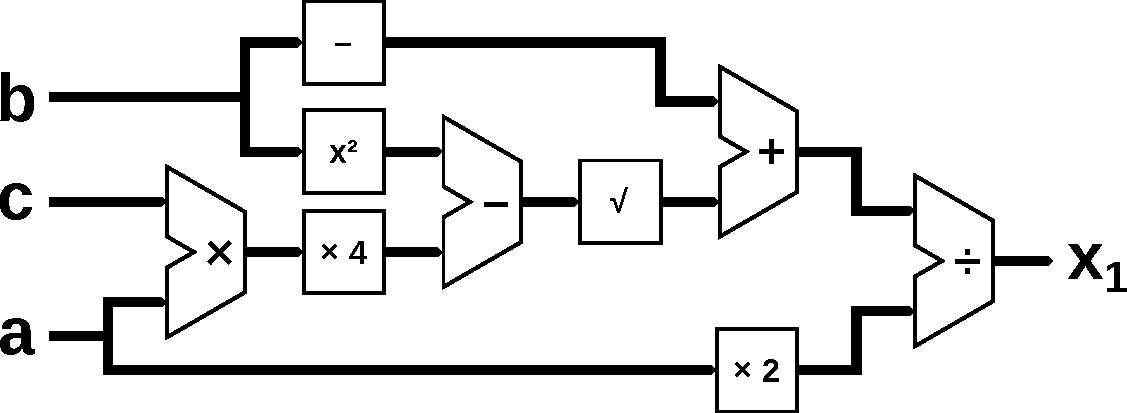
\includegraphics[width=\linewidth]{abc-formel.pdf}

        \[ x_1 = \frac{-b + \sqrt{b^2 - 4ac}}{2a} \]
      \end{center}
    \end{column}
    \begin{column}{.45\textwidth}
      Was fehlt?
      \begin{itemize}
      \item \textbf{Auswahl}\\
        $x_2$ ohne Neuverkabeln
      \item \textbf{Speicher}\\
        $a$, $b$, $c$ weg $\Rightarrow$ $x$ weg\quad :(
      \item \textbf{Programm}\\
        \texttt{goto}, \texttt{if}, \texttt{while}, \texttt{for}, \texttt{func}, \ldots
      \end{itemize}
    \end{column}
  \end{columns}
\end{frame}

\begin{frame}
  \frametitle{1/3: Auswahl}

  Wichtigstes Modul: \textbf{Multiplexer} (Spitzname: Mux)

  \begin{columns}
    \begin{column}{.45\textwidth}
      \begin{center}
        \begin{tabular}{cccc}
          \toprule
          select & in 0 & in 1 & out \\
          \midrule
          0 & 0 & 0 & 0 \\
          0 & 0 & 1 & 0 \\
          0 & 1 & 0 & 1 \\
          0 & 1 & 1 & 1 \\
          1 & 0 & 0 & 0 \\
          1 & 0 & 1 & 1 \\
          1 & 1 & 0 & 0 \\
          1 & 1 & 1 & 1 \\
          \bottomrule
        \end{tabular}
      \end{center}
    \end{column}
    \begin{column}{.45\textwidth}
      \begin{center}
        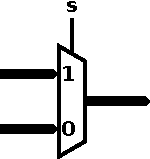
\includegraphics[width=.66\textwidth]{multiplexer.pdf}
      \end{center}
    \end{column}
  \end{columns}
\end{frame}

\begin{frame}
  \frametitle{Fast eine ALU}

    \begin{columns}[T]
    \begin{column}{.45\textwidth}
        \only<1>{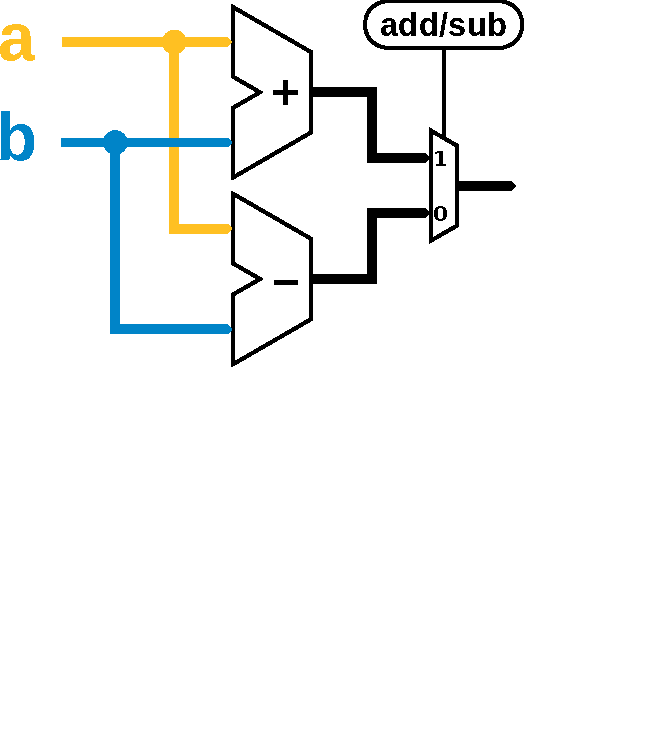
\includegraphics[height=\linewidth]{alu2.pdf}}
        \only<2>{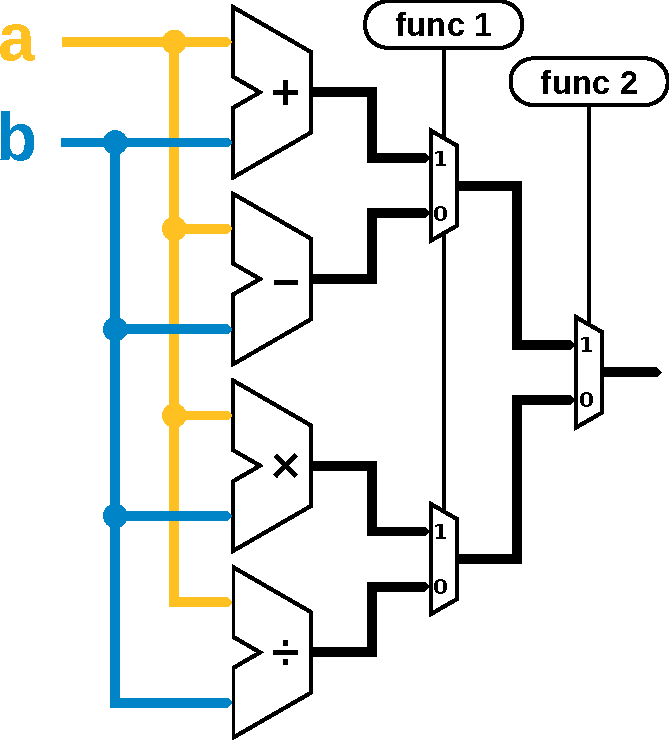
\includegraphics[height=\linewidth]{alu4.pdf}}
    \end{column}
    \begin{column}{.45\textwidth}
      Prinzip: Erst rechnen, dann aussuchen

      \bigskip

      \textbf{Kontrollsignale}

      \begin{itemize}
      \item Steuern Datenfluss, bei uns vor allem an Multiplexern
      \item Jetzt: \enquote{Schalter}
      \item Später: Programmieren
      \end{itemize}

      \bigskip

      \only<2>{
        \begin{itemize}
        \item Mehr Möglichkeiten: Mux-Baum bauen
        \item nicht \emph{ganz} realistisch
        \end{itemize}
      }
  \end{column}
  \end{columns}
\end{frame}

\begin{frame}
  \frametitle{2/3: Speicher}

  \begin{center}
    Flip-Flop, Inverter-Ring, bistabile Relais, Kondensatoren, Ringkerne, Flipdots \ldots

    \textit{Alles das Gleiche und sowieso nur Gefrickel!}
  \end{center}

  \bigskip

  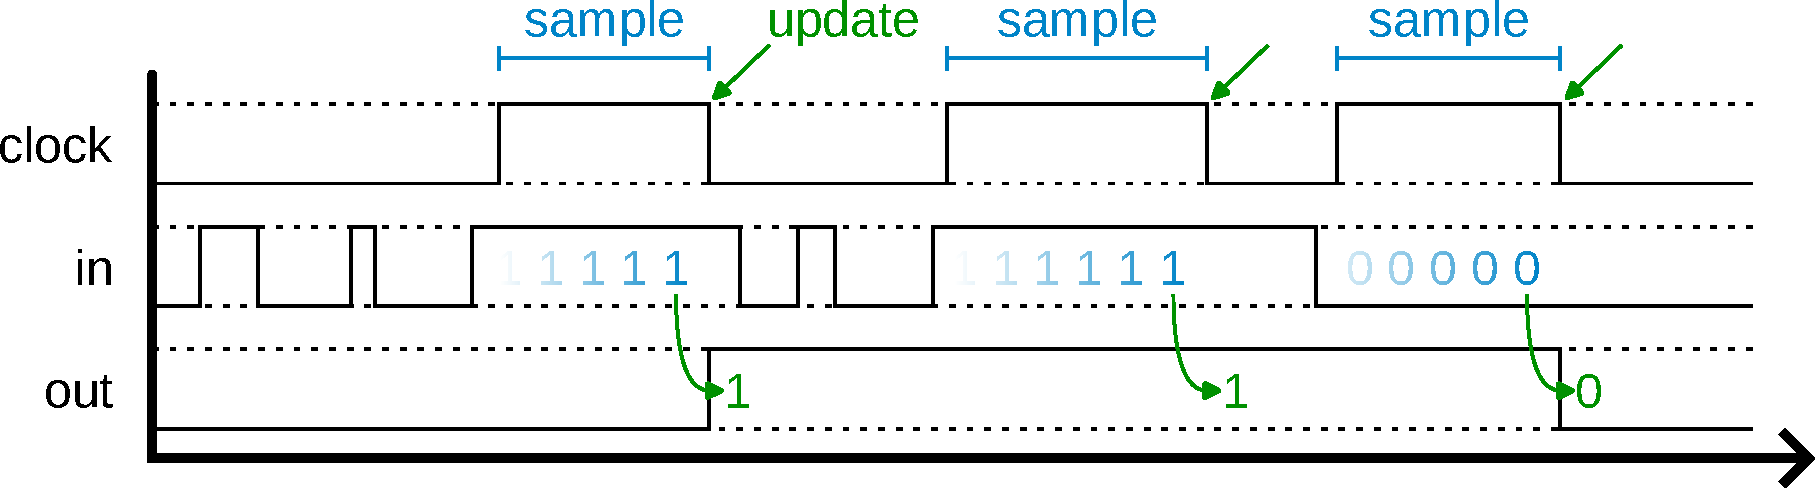
\includegraphics[width=\linewidth]{reg-waveform.pdf}
\end{frame}

\begin{frame}
  \frametitle{Speicher × 8}

  \begin{columns}[T]
    \begin{column}{.45\textwidth}
      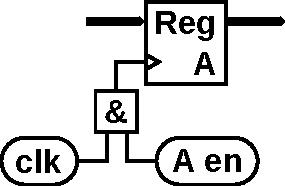
\includegraphics[width=\linewidth]{register.pdf}
    \end{column}
    \begin{column}{.45\textwidth}
      \begin{itemize}
      \item erstes Modul mit Takt\\
        Anschluss mit {\Large$\triangleright$}
      \item nicht immer jedes Register beschreiben\\
        $\Rightarrow$ \emph{Clock-Gate}
      \item Kontrollsignal \enquote{A enable}
      \end{itemize}
    \end{column}
  \end{columns}

\end{frame}

\begin{frame}
  \frametitle{\emph{mehr} Speicher}

  \begin{columns}
    \begin{column}{.7\textwidth}
      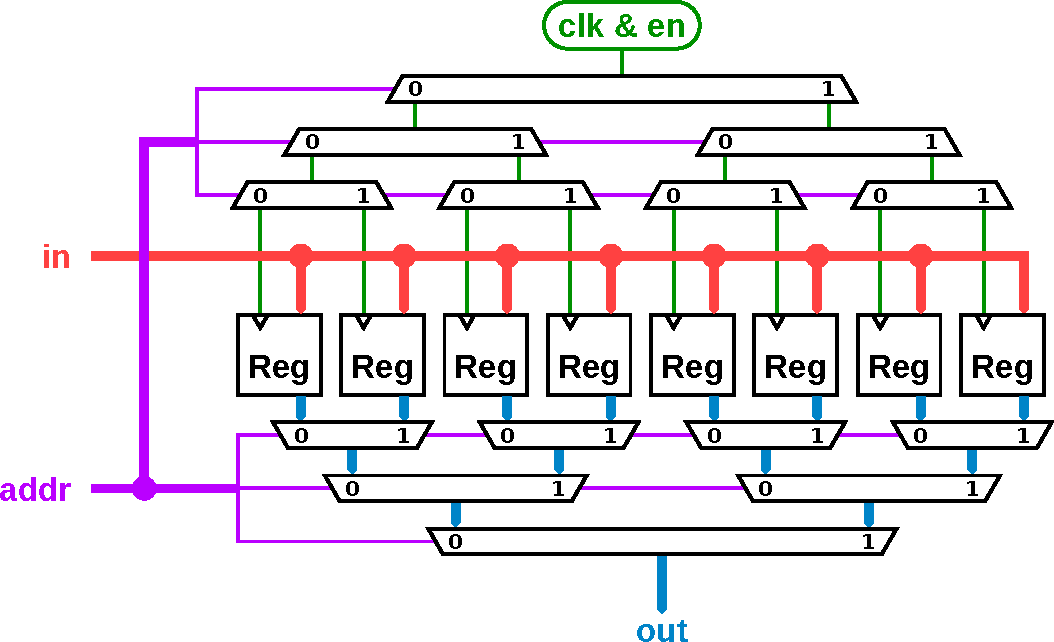
\includegraphics[width=\textwidth]{memory.pdf}
    \end{column}
    \begin{column}{.25\textwidth}
      \uncover<2>{Das wird \emph{groß}...}
    \end{column}
  \end{columns}

\end{frame}

\begin{frame}
  \frametitle{Leider gecheatet}

  \begin{itemize}
  \item 1 Register ${} \mathrel{\hat=} \qty{5}{\centi\metre} \times \qty{10}{\centi\metre}$
  \item 256 Register ($16 \times 16$) ${} \mathrel{\hat=} \qty{80}{\centi\metre} \times \qty{16}{\centi\metre}$
  \item \ldots von den Muxen ganz zu schweigen
  \end{itemize}

  \bigskip

  $\Rightarrow$ Geht nur mit Mikrochips

\end{frame}

\begin{frame}
  \frametitle{RAM}

  \begin{itemize}
  \item In jedem Takt Lesen \emph{oder} Schreiben
  \item Daten-Anschluss ist bidirektional $\Rightarrow$ etwas verdächtiger Mux
  \end{itemize}

  \bigskip

  \begin{center}
    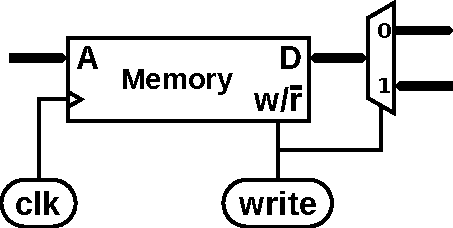
\includegraphics[width=.5\linewidth]{ram.pdf}
  \end{center}
\end{frame}

\begin{frame}
  \frametitle{Jetzt geht's los}

  Alles beisammen:

  \bigskip

  \renewcommand{\arraystretch}{3.5}

  \begin{tabular}{clc>{\qquad}clc}
    \setcounter{enumi}{1}\usebeamertemplate{enumerate item}
    & Berechnungen
    & 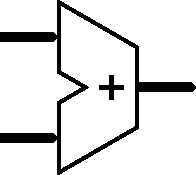
\includegraphics[align=c,height=3em]{adder.pdf}
    & \setcounter{enumi}{1}\usebeamertemplate{enumerate item}
    & Speicher
    & 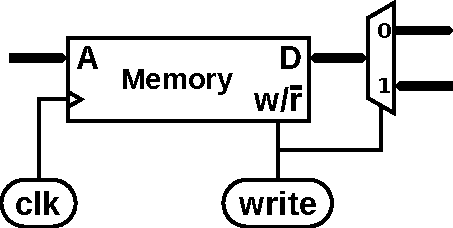
\includegraphics[align=c,height=3em]{ram.pdf} \\

    \setcounter{enumi}{2}\usebeamertemplate{enumerate item}
    & Multiplexer
    & 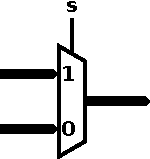
\includegraphics[align=c,height=3em]{multiplexer.pdf}
    & \setcounter{enumi}{5}\usebeamertemplate{enumerate item}
    & \multicolumn{2}{l}{???\qquad{}\uncover<2>{\textbf{$\leftblackarrow$ Sie befinden sich hier}}}
    \\

    \setcounter{enumi}{3}\usebeamertemplate{enumerate item}
    & Register
    & 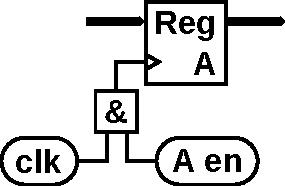
\includegraphics[align=c,height=3em]{register.pdf}
    & \setcounter{enumi}{6}\usebeamertemplate{enumerate item}
    & \cancel{Profit} Prozessor
    &
  \end{tabular}
\end{frame}

\begin{frame}
  \frametitle{Assembler}

  Wie sollen Instruktionen aussehen?
  \begin{itemize}
  \item Wie RISC (ARM, RISC-V, MIPS, SPARC, \ldots): \texttt{add r3, r2, r1}\\
    16/32 Register, 3 Register in jeder Instruktion, Laden/Speichern anderes Format
  \item Wie x86: \texttt{addq \%rsi, 42(\%rbx, \%rcx, 4)}\\
    Nein
  \item Wie 6502: \texttt{lda \$23; adc \$42}\\
    4(?) Register, 1 Operand, (fast) immer genau ein Speicherzugriff\\
    \pause
    \textbf{Das klingt gut!}
  \end{itemize}

  \bigskip

  Unser Plan:
  \begin{itemize}
  \item Opcode + 1 Operand
  \item wenige Register
  \item einmal Laden/Speichern pro Instruktion
  \end{itemize}

\end{frame}

\begin{frame}
  \frametitle{Akkumulator-Architektur}

  \begin{itemize}
  \item \emph{ein einziges} Register (\texttt{A})
  \item alle Berechnungen \enquote{\texttt{A} $\circledast$ Speicher}
  \item ein Speicherzugriff pro Instruktion $\checkmark$
  \end{itemize}

  \bigskip

  \texttt{z = x + y;} wird zu

  \bigskip

  {\Large
    \texttt{load~~\&x} \qquad \texttt{A = x};\\
    \texttt{add~~~\&y} \qquad \texttt{A = A + y;}\\
    \texttt{store~\&z} \qquad \texttt{z = A;}\\
  }
\end{frame}

\begin{frame}
  \frametitle{ALU-Aufbau: Rechnungen}

  \strut{}ALU + Write-Back in den Akkumulator

  \begin{center}
    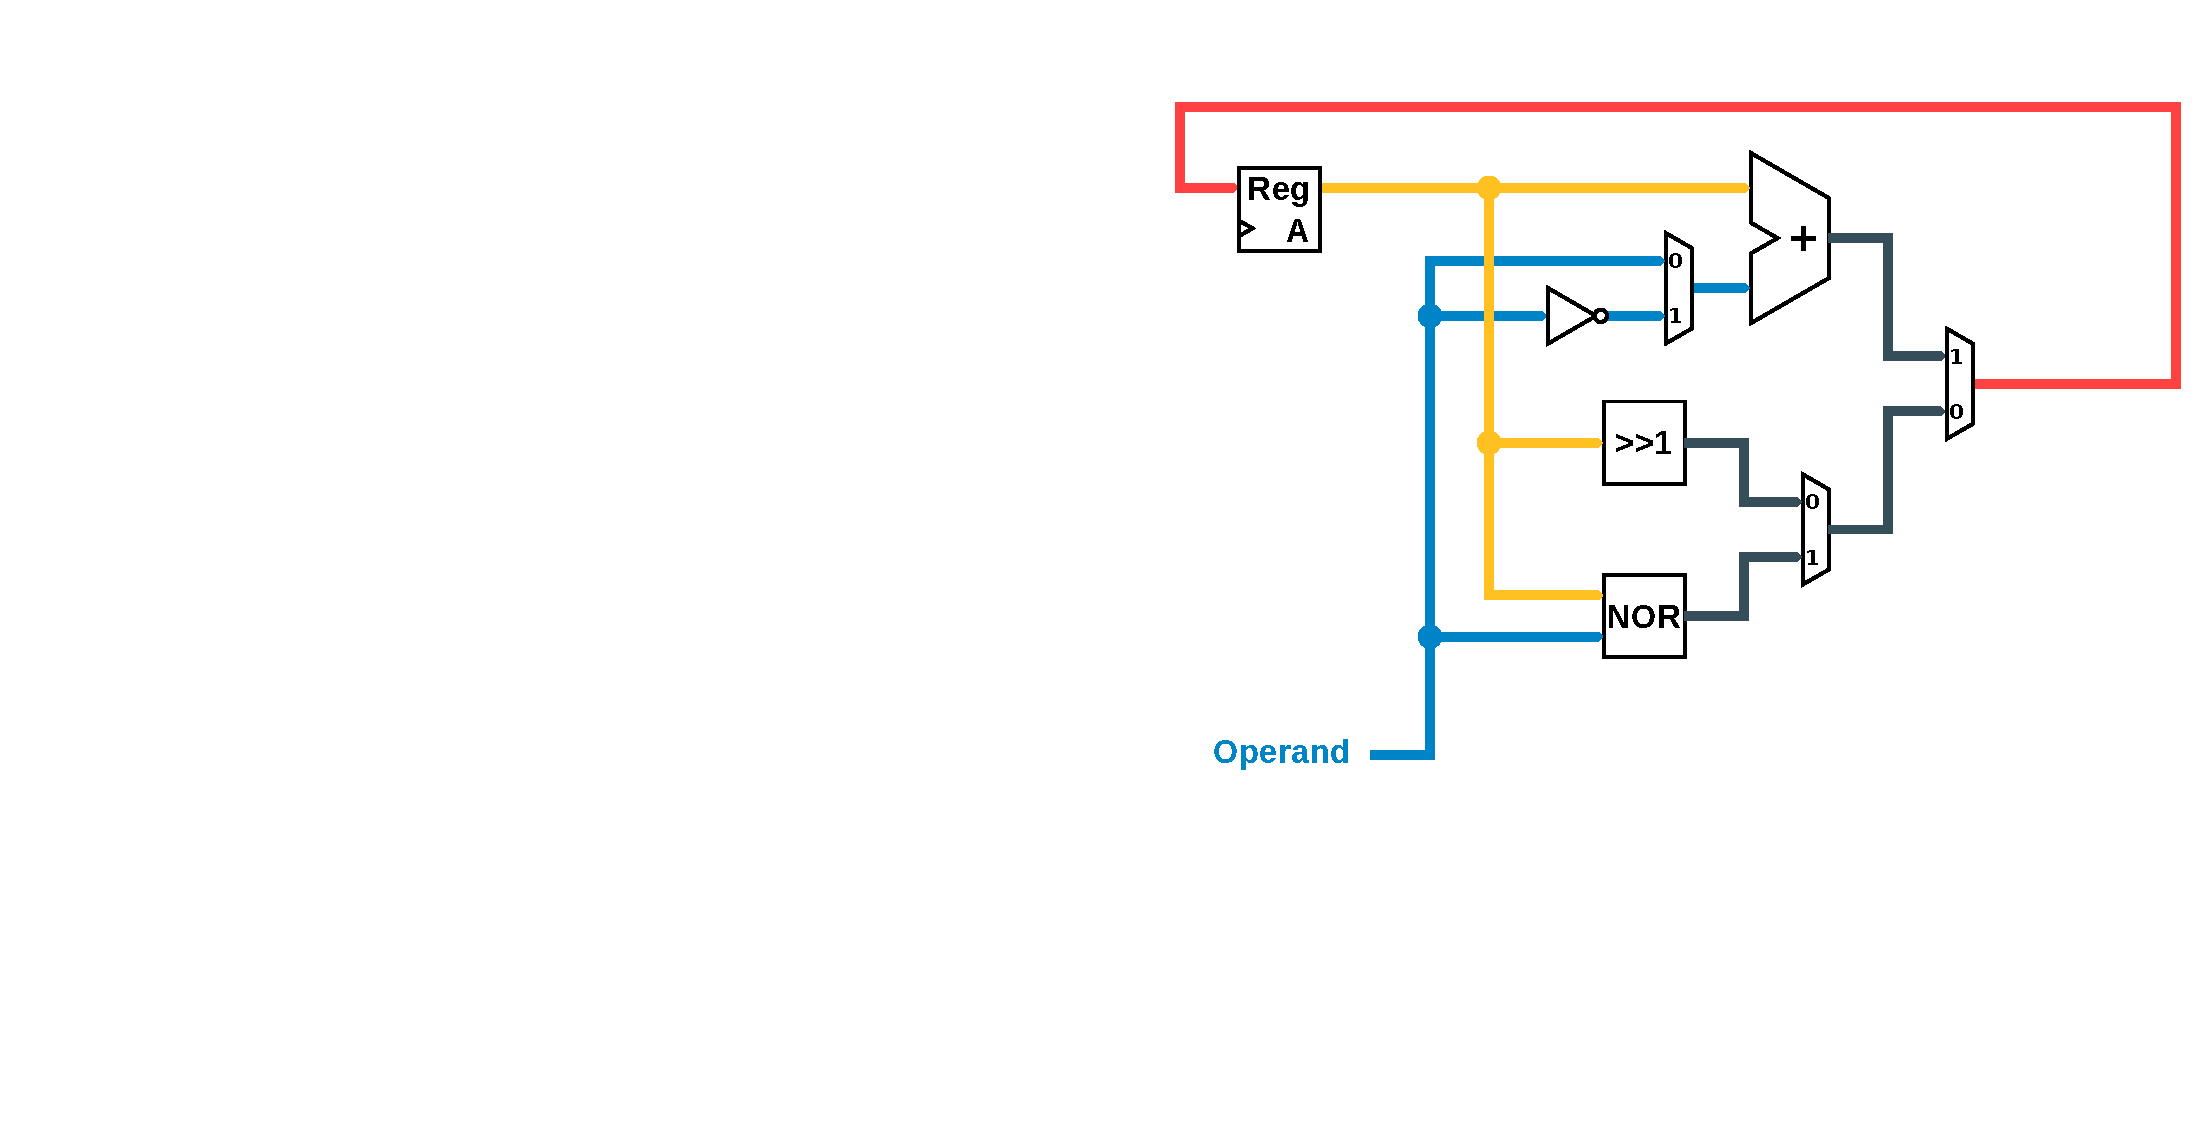
\includegraphics[width=.85\textwidth]{sch-alu.pdf}
  \end{center}
\end{frame}

\begin{frame}
  \frametitle{ALU-Aufbau: \texttt{load}}

  \strut{}Ein Weg an der ALU vorbei um Daten in A zu laden

  \begin{center}
    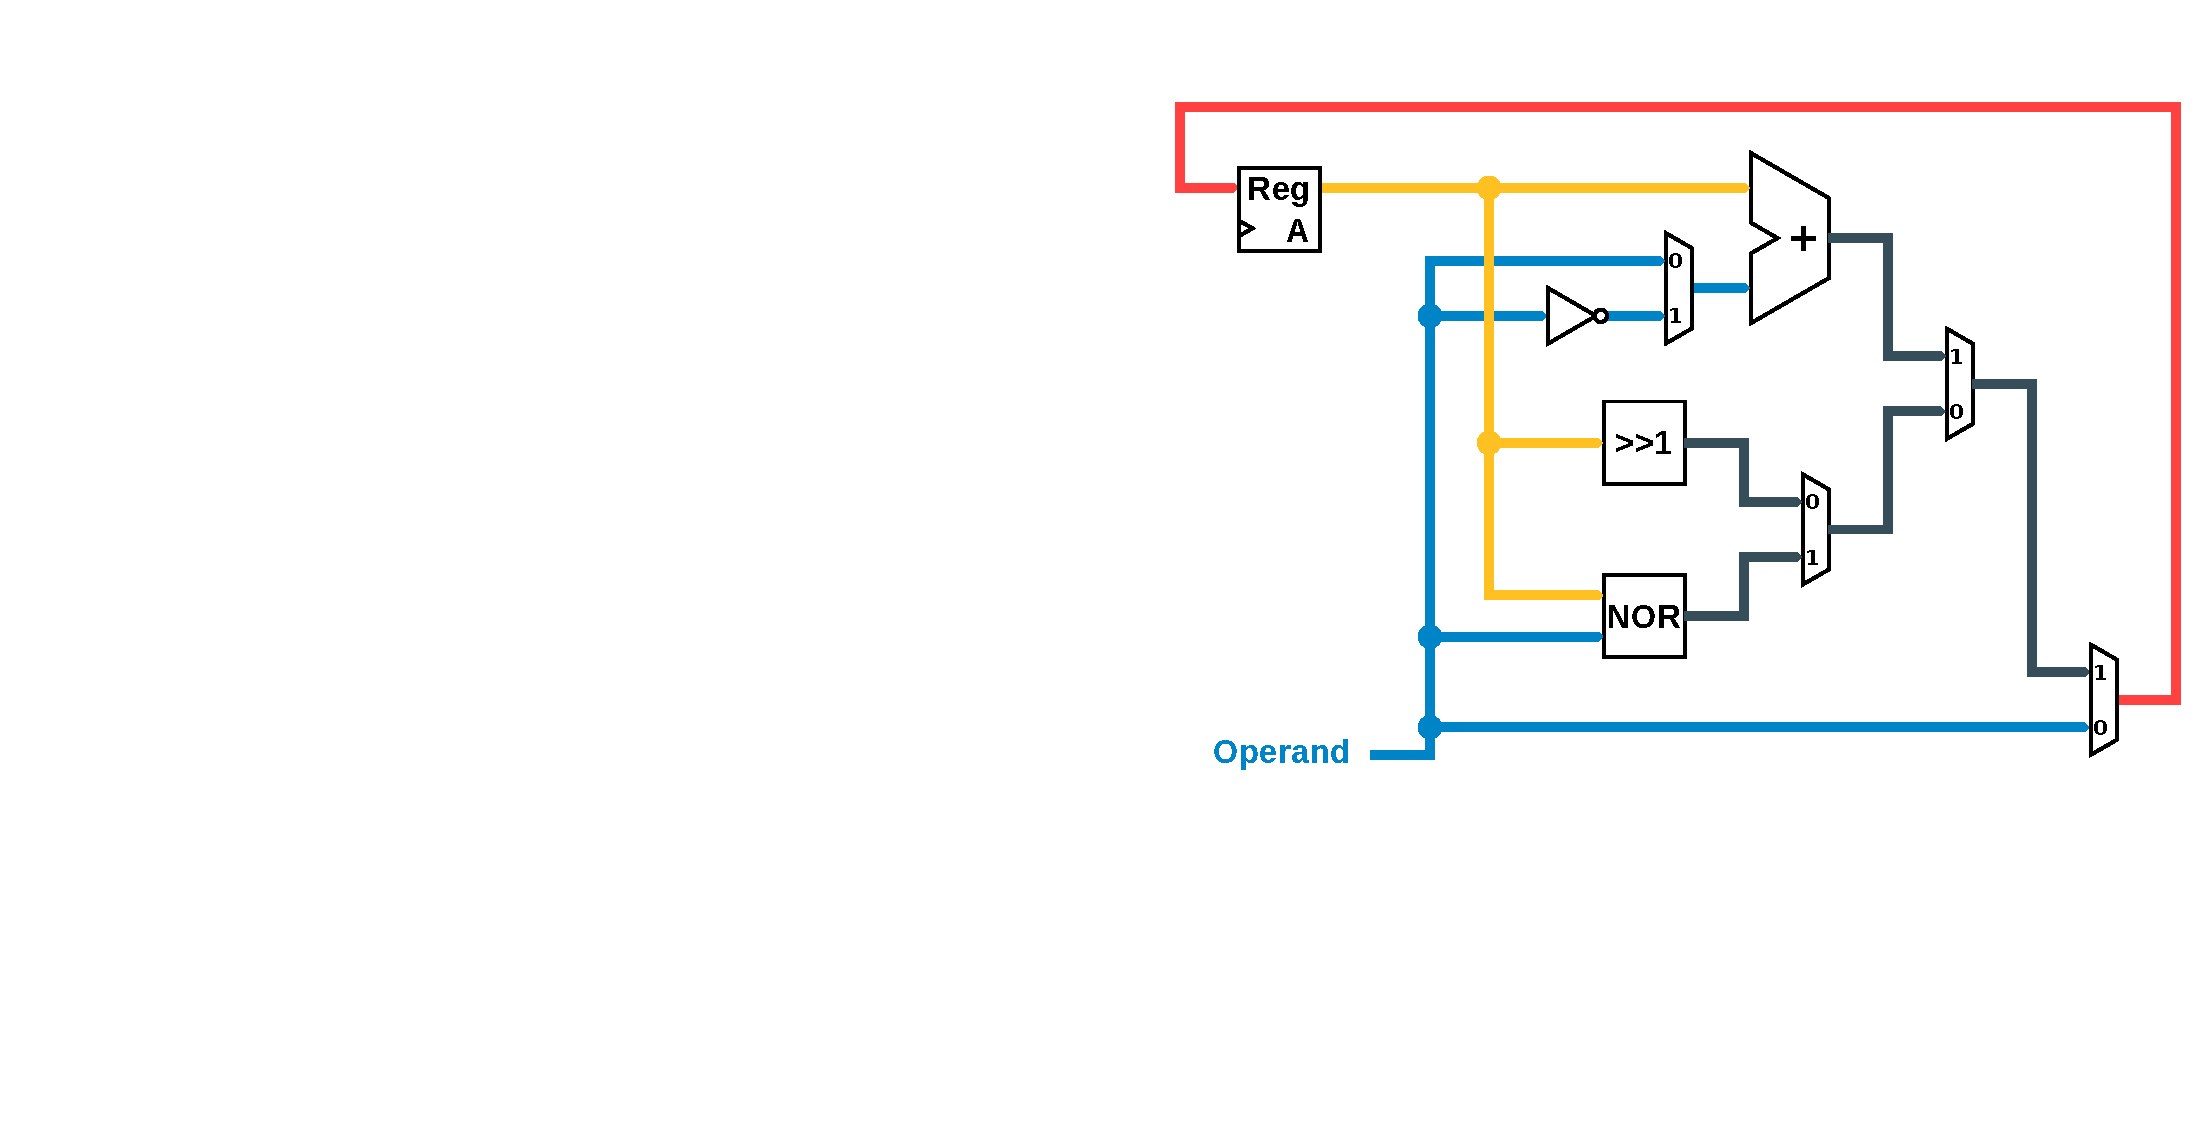
\includegraphics[width=.85\textwidth]{sch-load.pdf}
  \end{center}
\end{frame}

\begin{frame}
  \frametitle{ALU-Aufbau: \texttt{store}}

  \strut{}Ergebnisse müssen in den Speicher zurück

  \begin{center}
    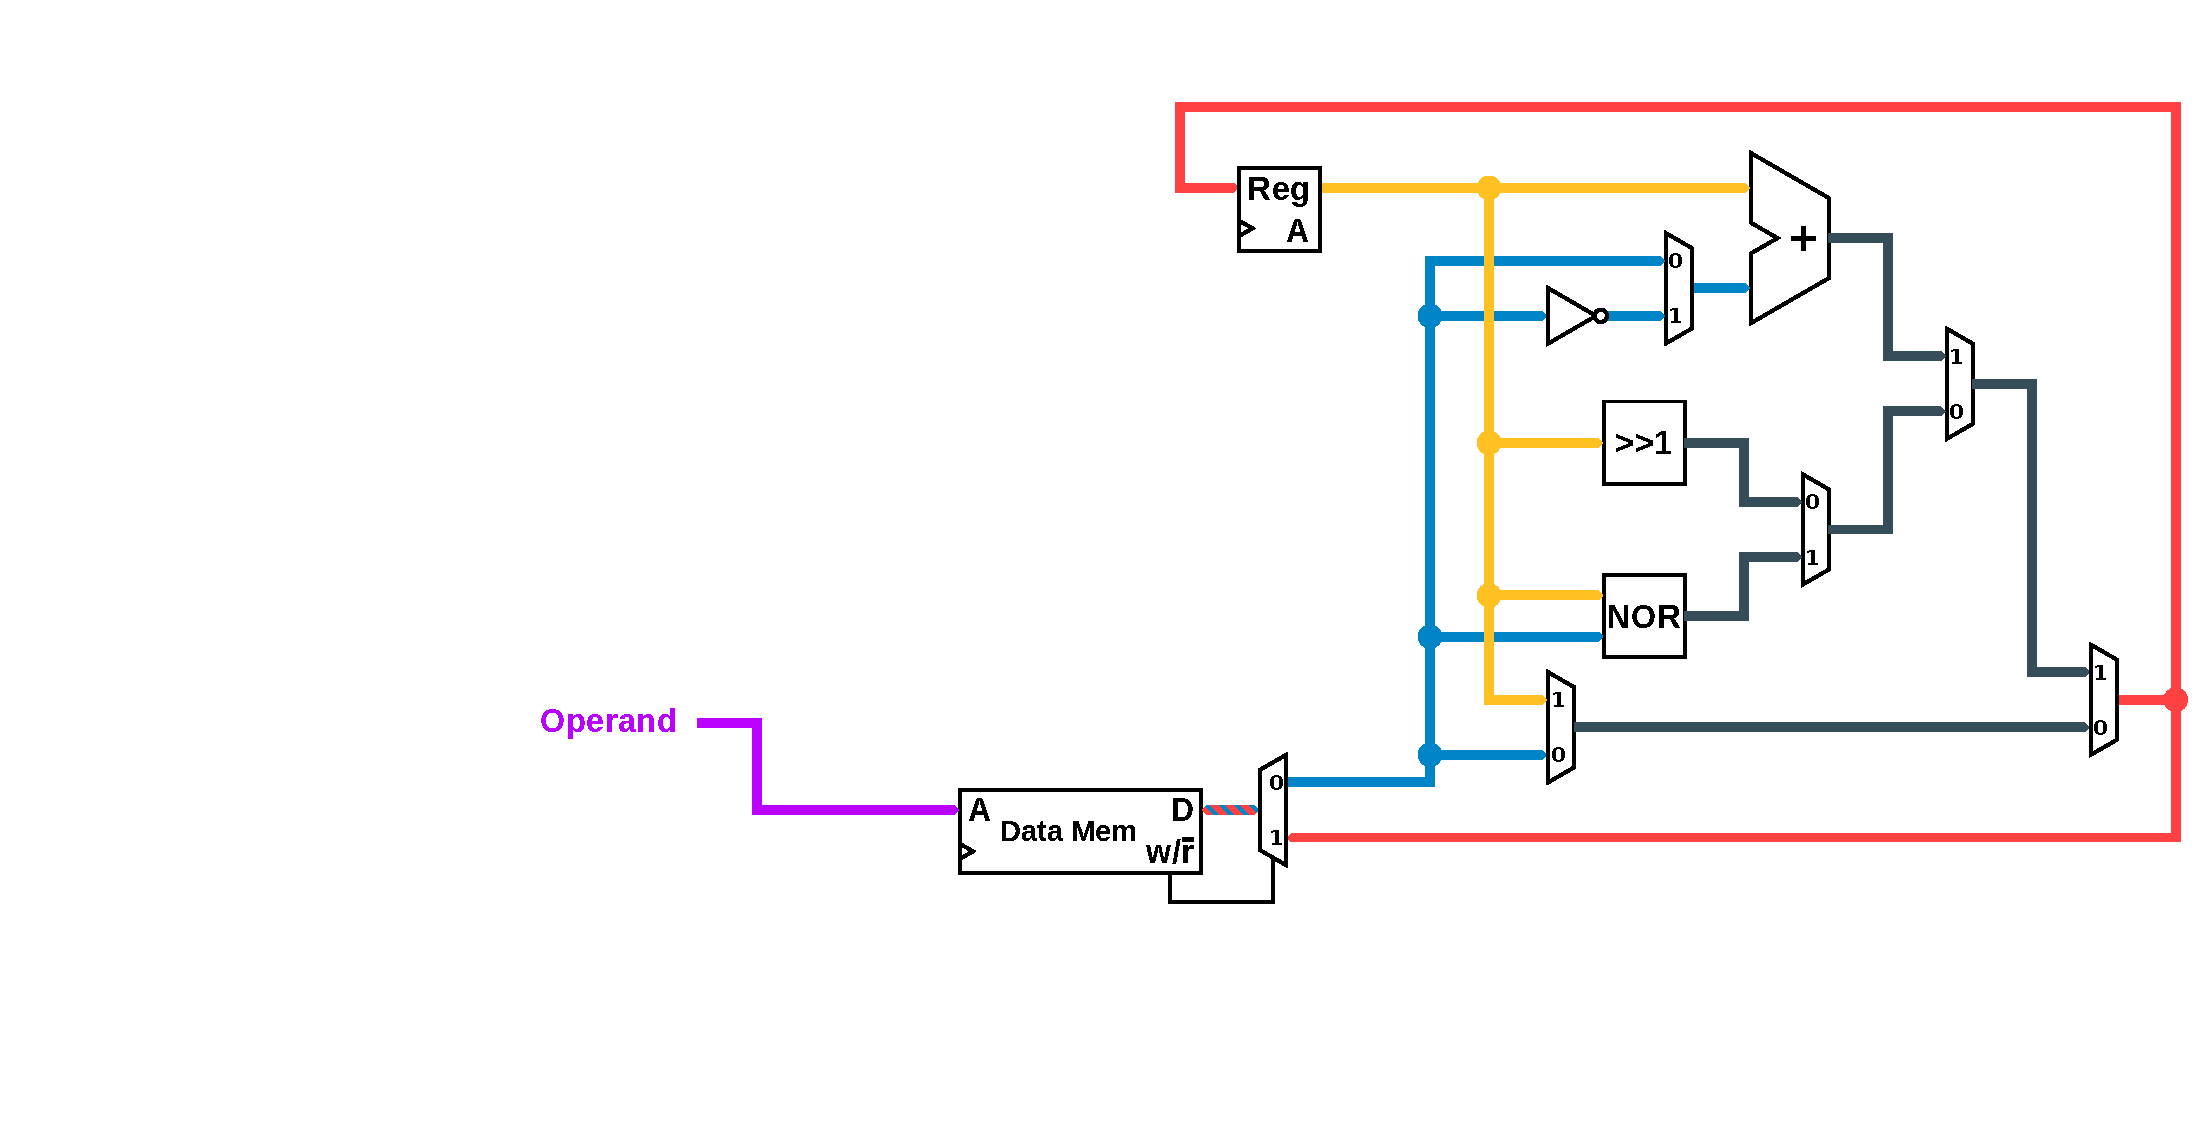
\includegraphics[width=.85\textwidth]{sch-loadstore.pdf}
  \end{center}
\end{frame}

\begin{frame}
  \frametitle{Immediates}

  Konstanten sind auch wichtig:
  \begin{itemize}
  \item \texttt{answer = secret + 19;}
  \item \texttt{start = 0;}
  \item \texttt{i++}
  \end{itemize}

  \bigskip

  In Assembler \enquote{Immediate}. Operand als Wert, nicht als Adresse

  \medskip

  {\Large
    \begin{tabular}{ll}
      \texttt{add 19} & \texttt{addi 19} \\
      \texttt{load 0} & \texttt{loadi 0} \\
    \end{tabular}
  }

  \bigskip

  \pause
  Wir brauchen noch ein Mux \ldots\ (es wird nicht das Letzte sein)
\end{frame}

\begin{frame}
  \frametitle{Immediates}

  \strut{}Operand direkt in die ALU geben

  \begin{center}
    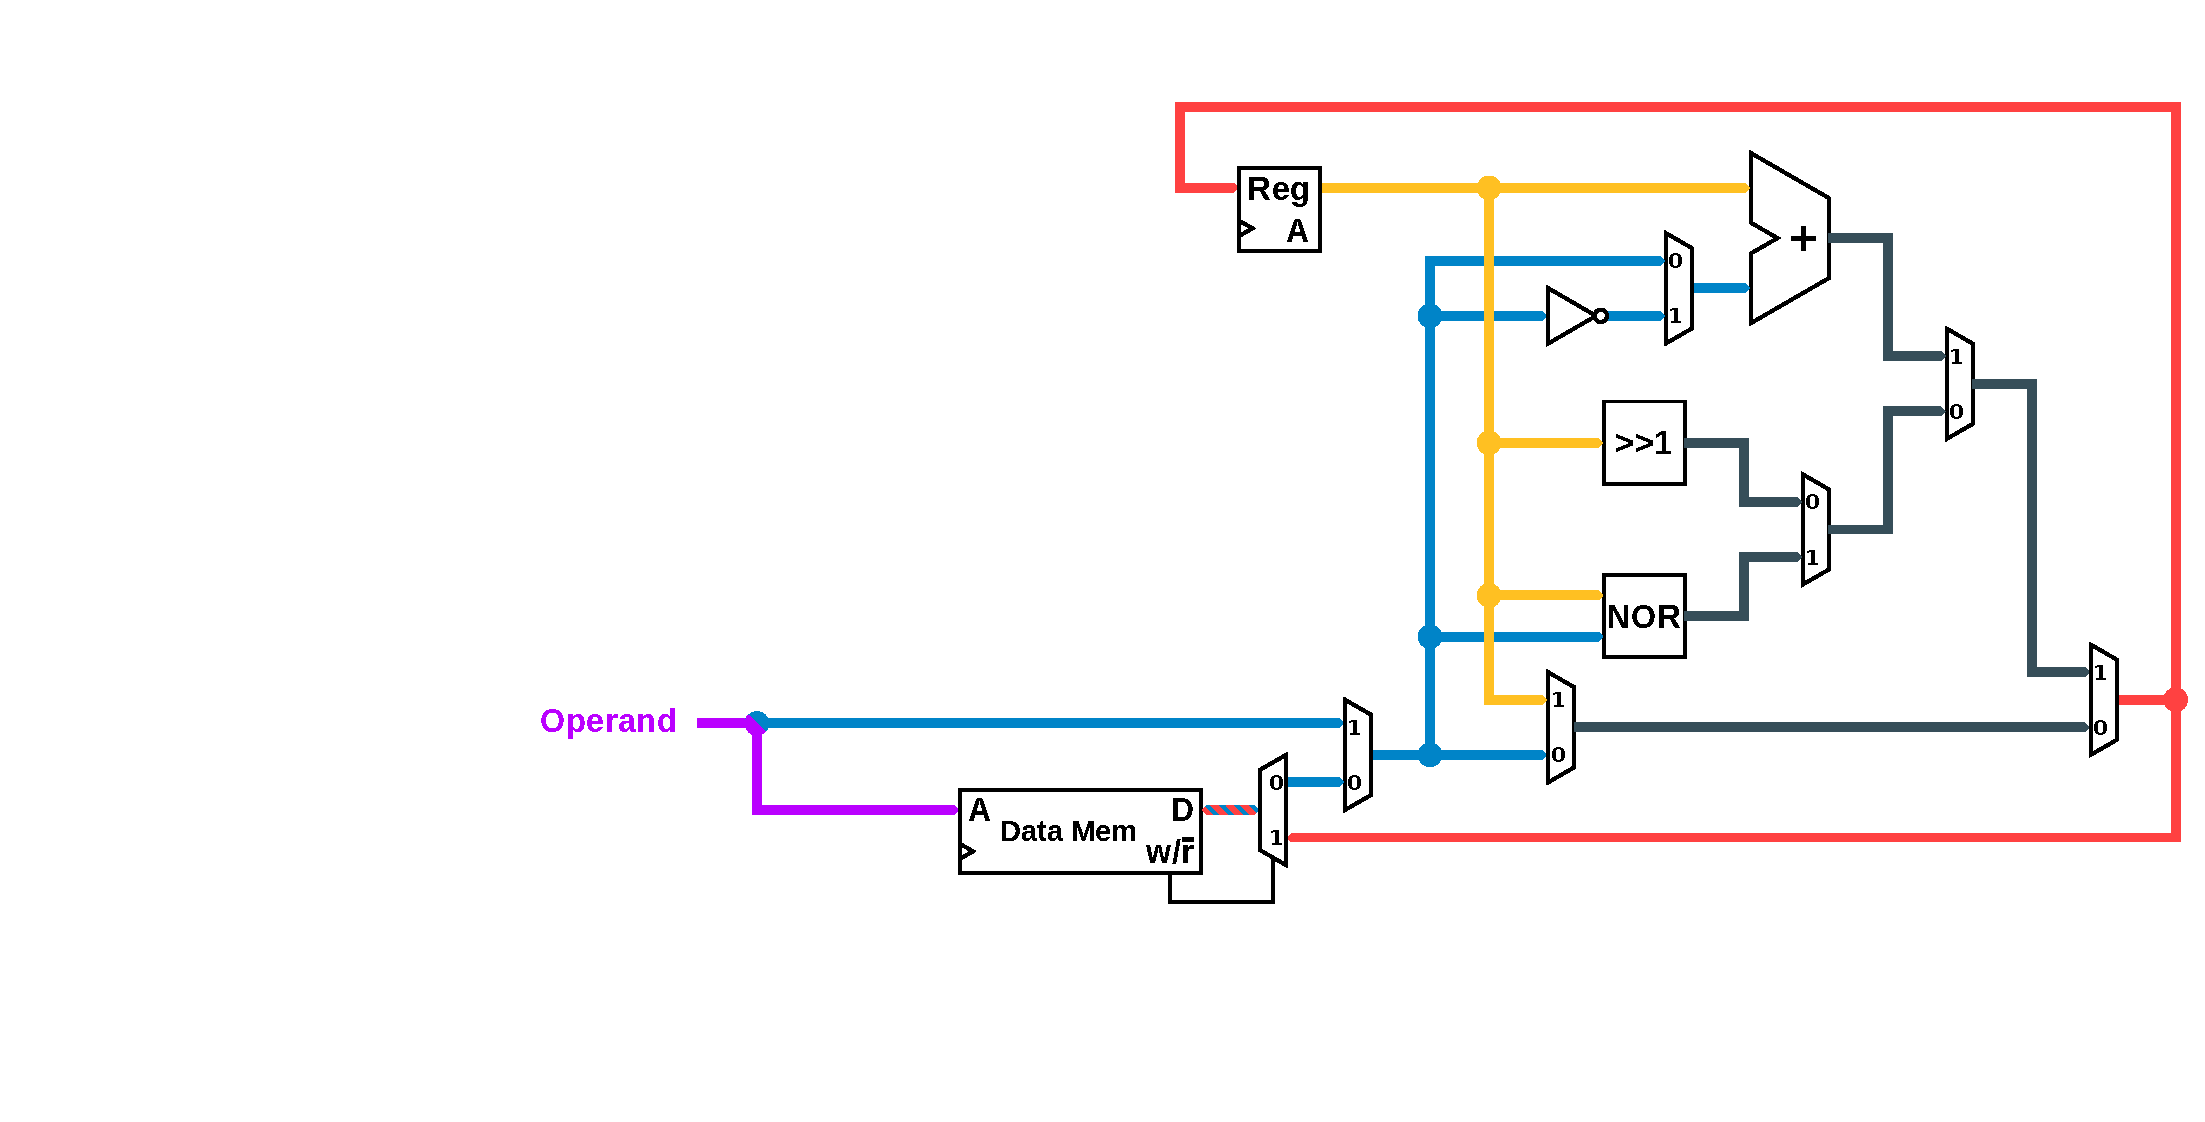
\includegraphics[width=.85\textwidth]{sch-immediate.pdf}
  \end{center}
\end{frame}

\begin{frame}
  \frametitle{Pointer}

  Manchmal sind Adressen nicht fest:
  \begin{itemize}
  \item \texttt{int *p = lol(); int x = *p;}
  \item \texttt{cpu->bits = 8;}
  \item \texttt{dinge[i] = d;}
  \end{itemize}

  \bigskip

  Adresse in A berechnen und dann Laden/Speichern?\\
  Nope: \texttt{*p = x;} braucht \texttt{p} und \texttt{x} gleichzeitig

  \bigskip
  \pause

  Wir brauchen noch ein Mux und ein \emph{Register} \ldots\ (zum Glück das Vorletzte)

\end{frame}

\begin{frame}
  \frametitle{Pointer}

  \strut{}Zweites Register mit Write-Back, Auswahl der Datenadresse

  \begin{center}
    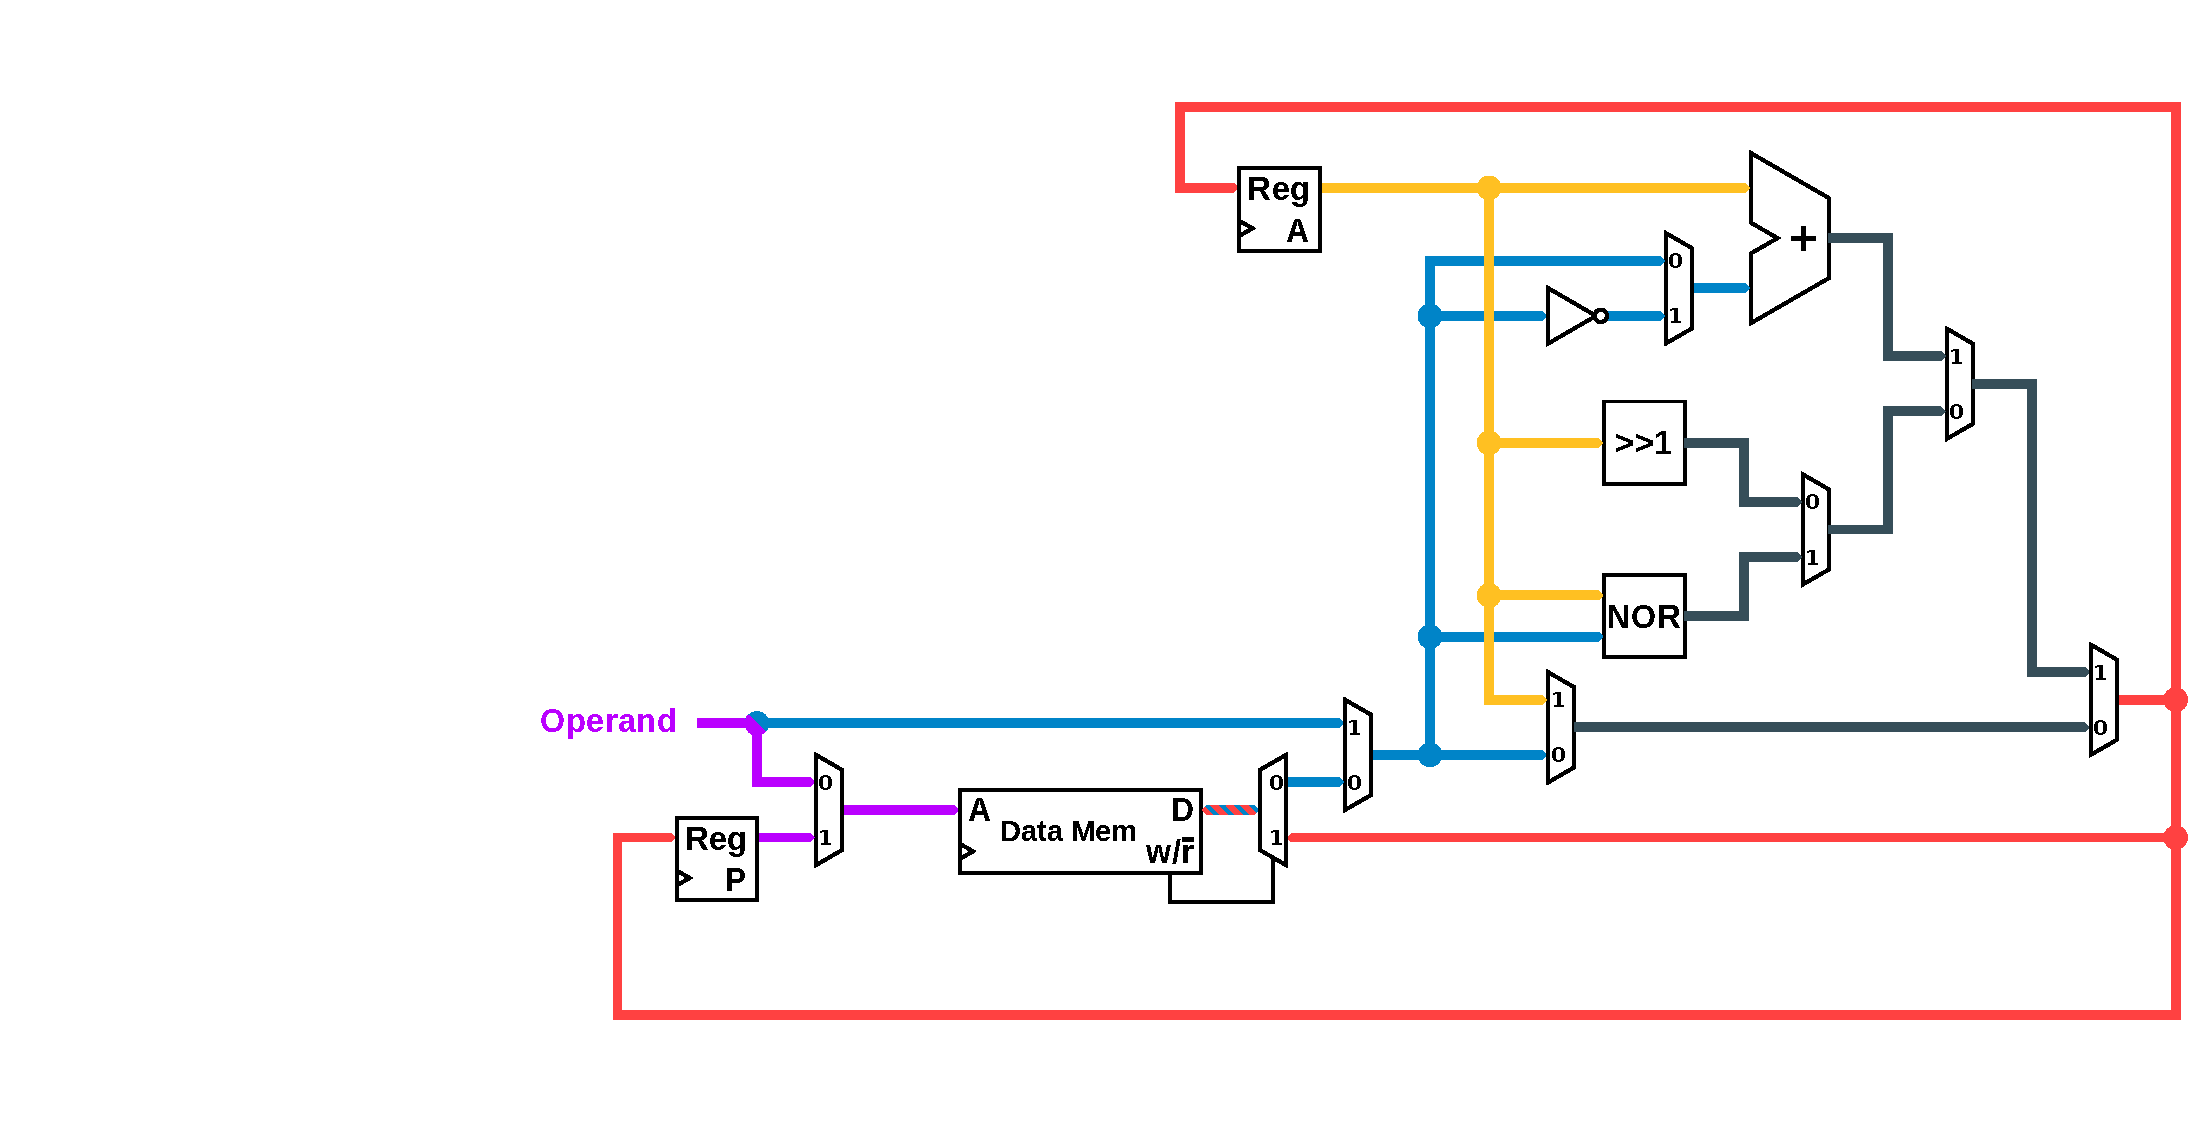
\includegraphics[width=.85\textwidth]{sch-pointer.pdf}
  \end{center}
\end{frame}

\begin{frame}
  \frametitle{Fertig ist der \emph{Data-Path}}

  \strut{}\alt<2>{\cancel{9} 8}{9} Kontrollsignale steuern alles

  \begin{center}
    \alt<2>{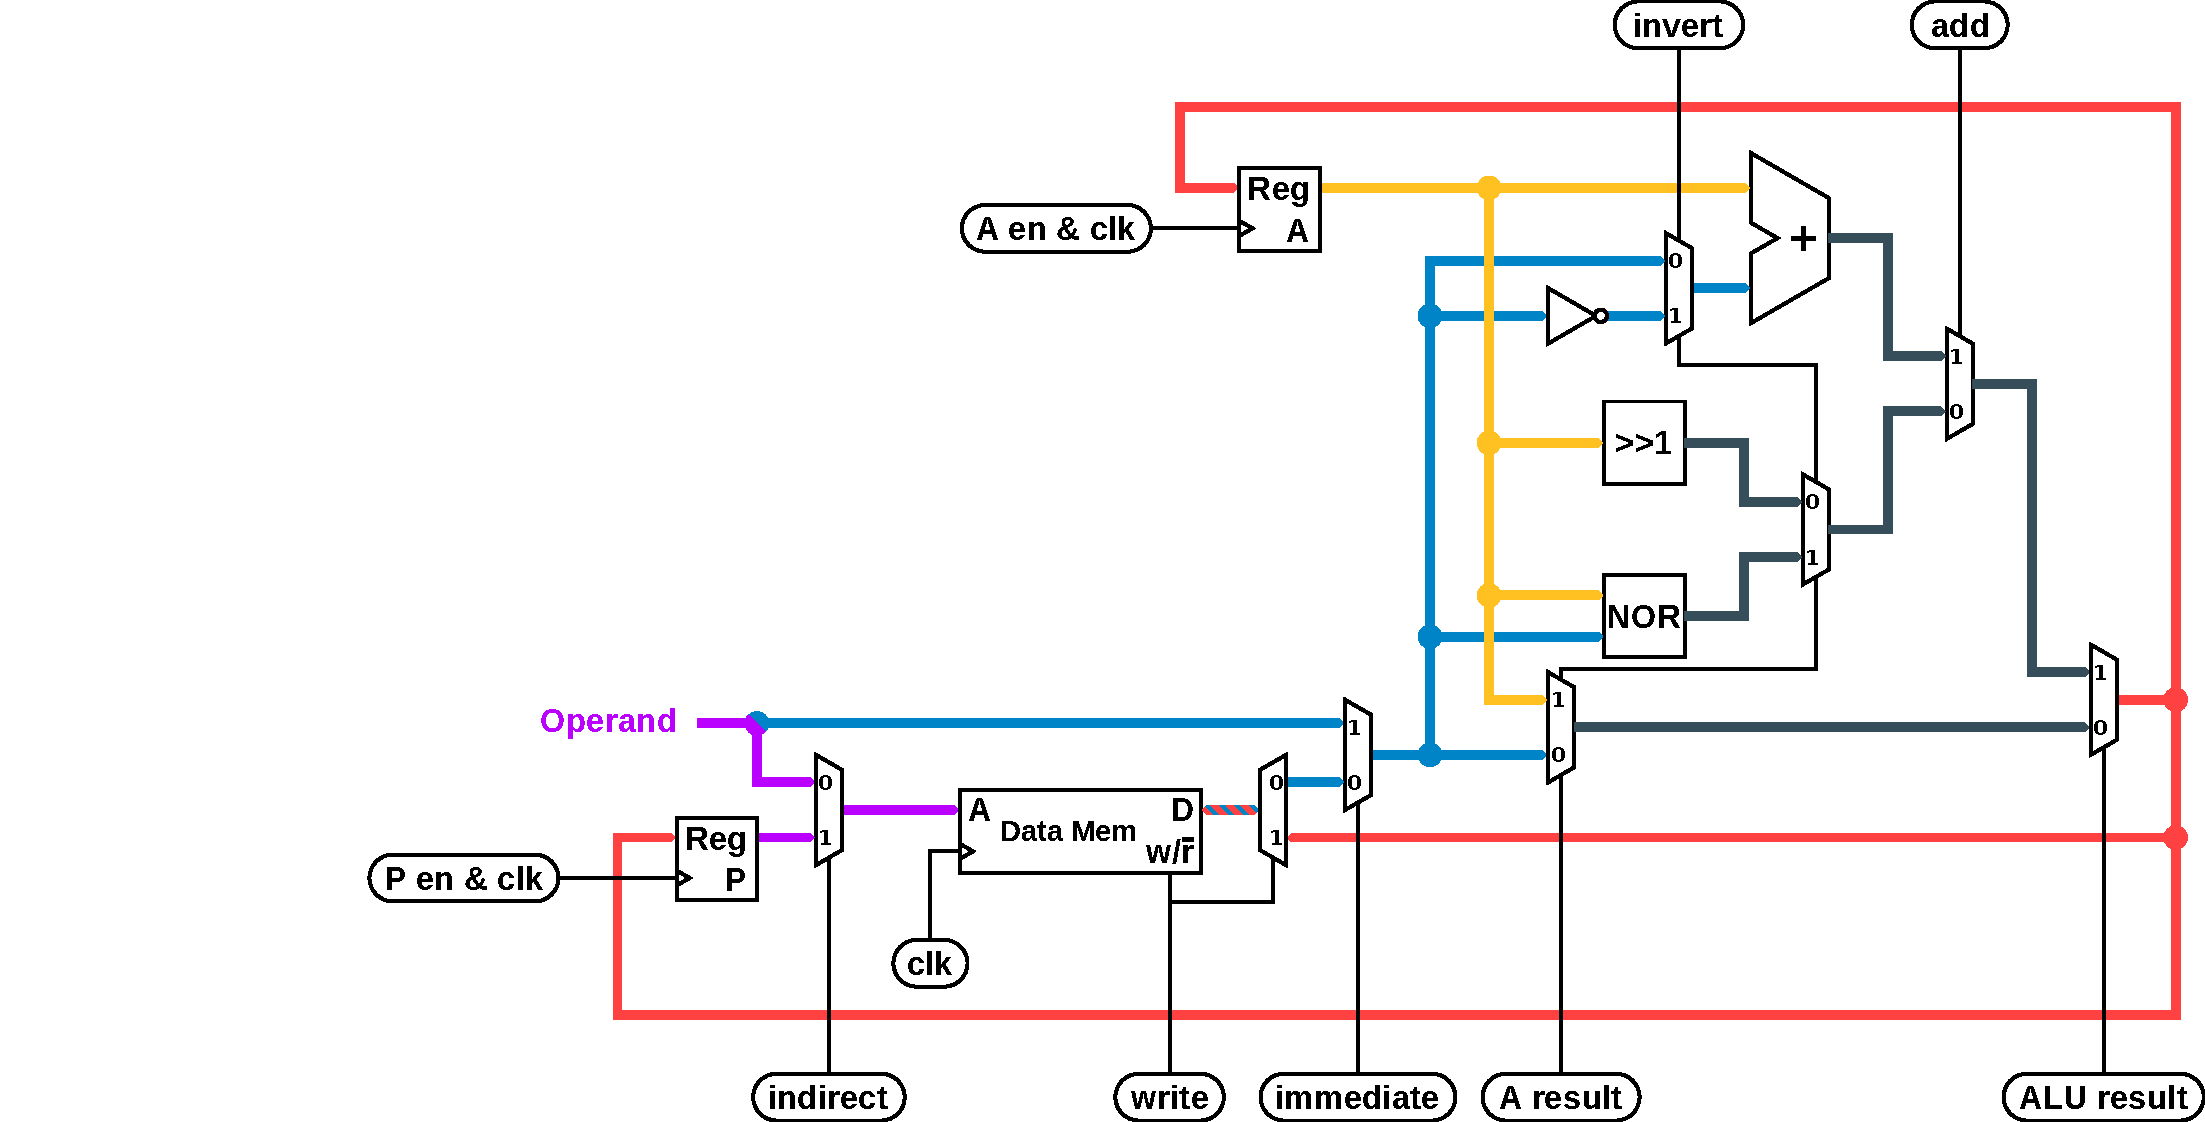
\includegraphics[width=.85\textwidth]{sch-controls2.pdf}}{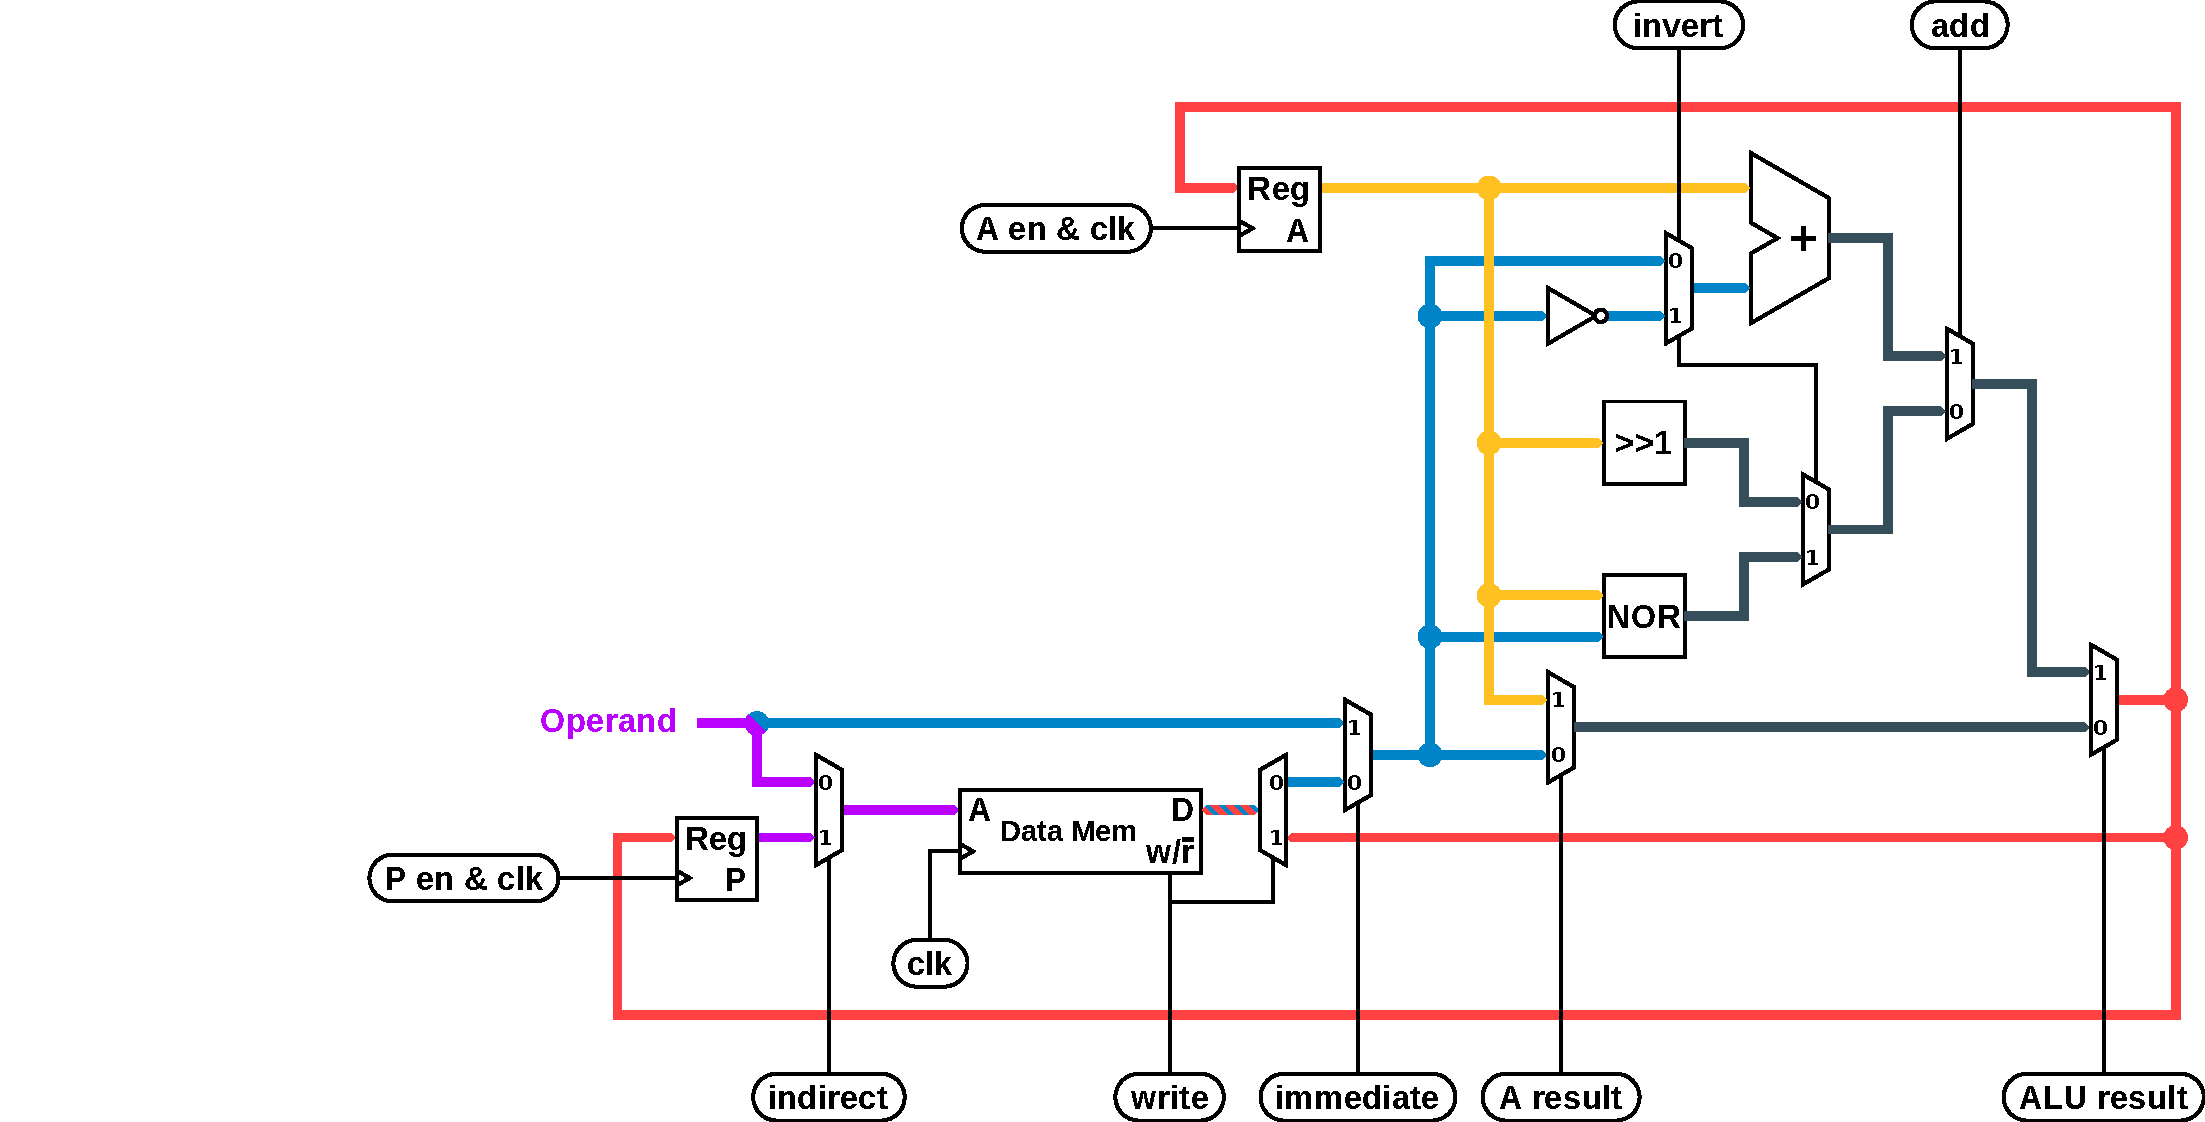
\includegraphics[width=.85\textwidth]{sch-controls.pdf}}
  \end{center}
\end{frame}

\begin{frame}
  \frametitle{Plötzlich Maschinencode}

  {\centering
    \begin{tikzpicture}
      \node[draw,thick,minimum width=5em,minimum height=5em,align=center] at (0,0) {\footnotesize Speicher\\\footnotesize schreiben};
      \node[draw,thick,minimum width=5em,minimum height=5em,align=center] at (5em,0) {\footnotesize Reg. P\\\footnotesize schreiben};
      \node[draw,thick,minimum width=5em,minimum height=5em,align=center] at (10em,0) {\footnotesize Reg. A\\\footnotesize schreiben};
      \node[draw,thick,minimum width=5em,minimum height=5em,align=center] at (15em,0) {\footnotesize ALU\\\footnotesize benutzen};
      \node[draw,thick,minimum width=5em,minimum height=5em,align=center] at (20em,0) {\footnotesize A lesen\\\footnotesize ——\\\footnotesize \enquote{invertieren}};
      \node[draw,thick,minimum width=5em,minimum height=5em,align=center] at (25em,0) {\footnotesize Addierer\\\footnotesize benutzen};
      \node[draw,thick,minimum width=5em,minimum height=5em,align=center] at (30em,0) {\footnotesize Immediate};
      \node[draw,thick,minimum width=5em,minimum height=5em,align=center] at (35em,0) {\footnotesize Indirekt};
    \end{tikzpicture}
  }

  \begin{itemize}
  \item Eine Mux-Einstellung $\hat=$ ein Bit $\Rightarrow$ 8 in einem Byte zusammenfassen
  \item z.B. \texttt{add}: A schreiben, Ergebnis von der ALU, Addierer benutzen, sonst nichts\\
    $\Rightarrow \mathtt{add} = \text{0b00110100} = \text{0x34}$

    \medskip

  \item Zweites Byte für den Operanden: $\mathtt{add~42} = \text{0x342a}$
  \end{itemize}

  \bigskip

  \pause

  Eine Instruktion = 16 bit $\Rightarrow$ \textbf{Das können wir speichern!}
\end{frame}

\begin{frame}
  \frametitle{Programmspeicher}

  \strut{}Noch ein Speicher für das Programm (\enquote{Harvard})

  \begin{center}
    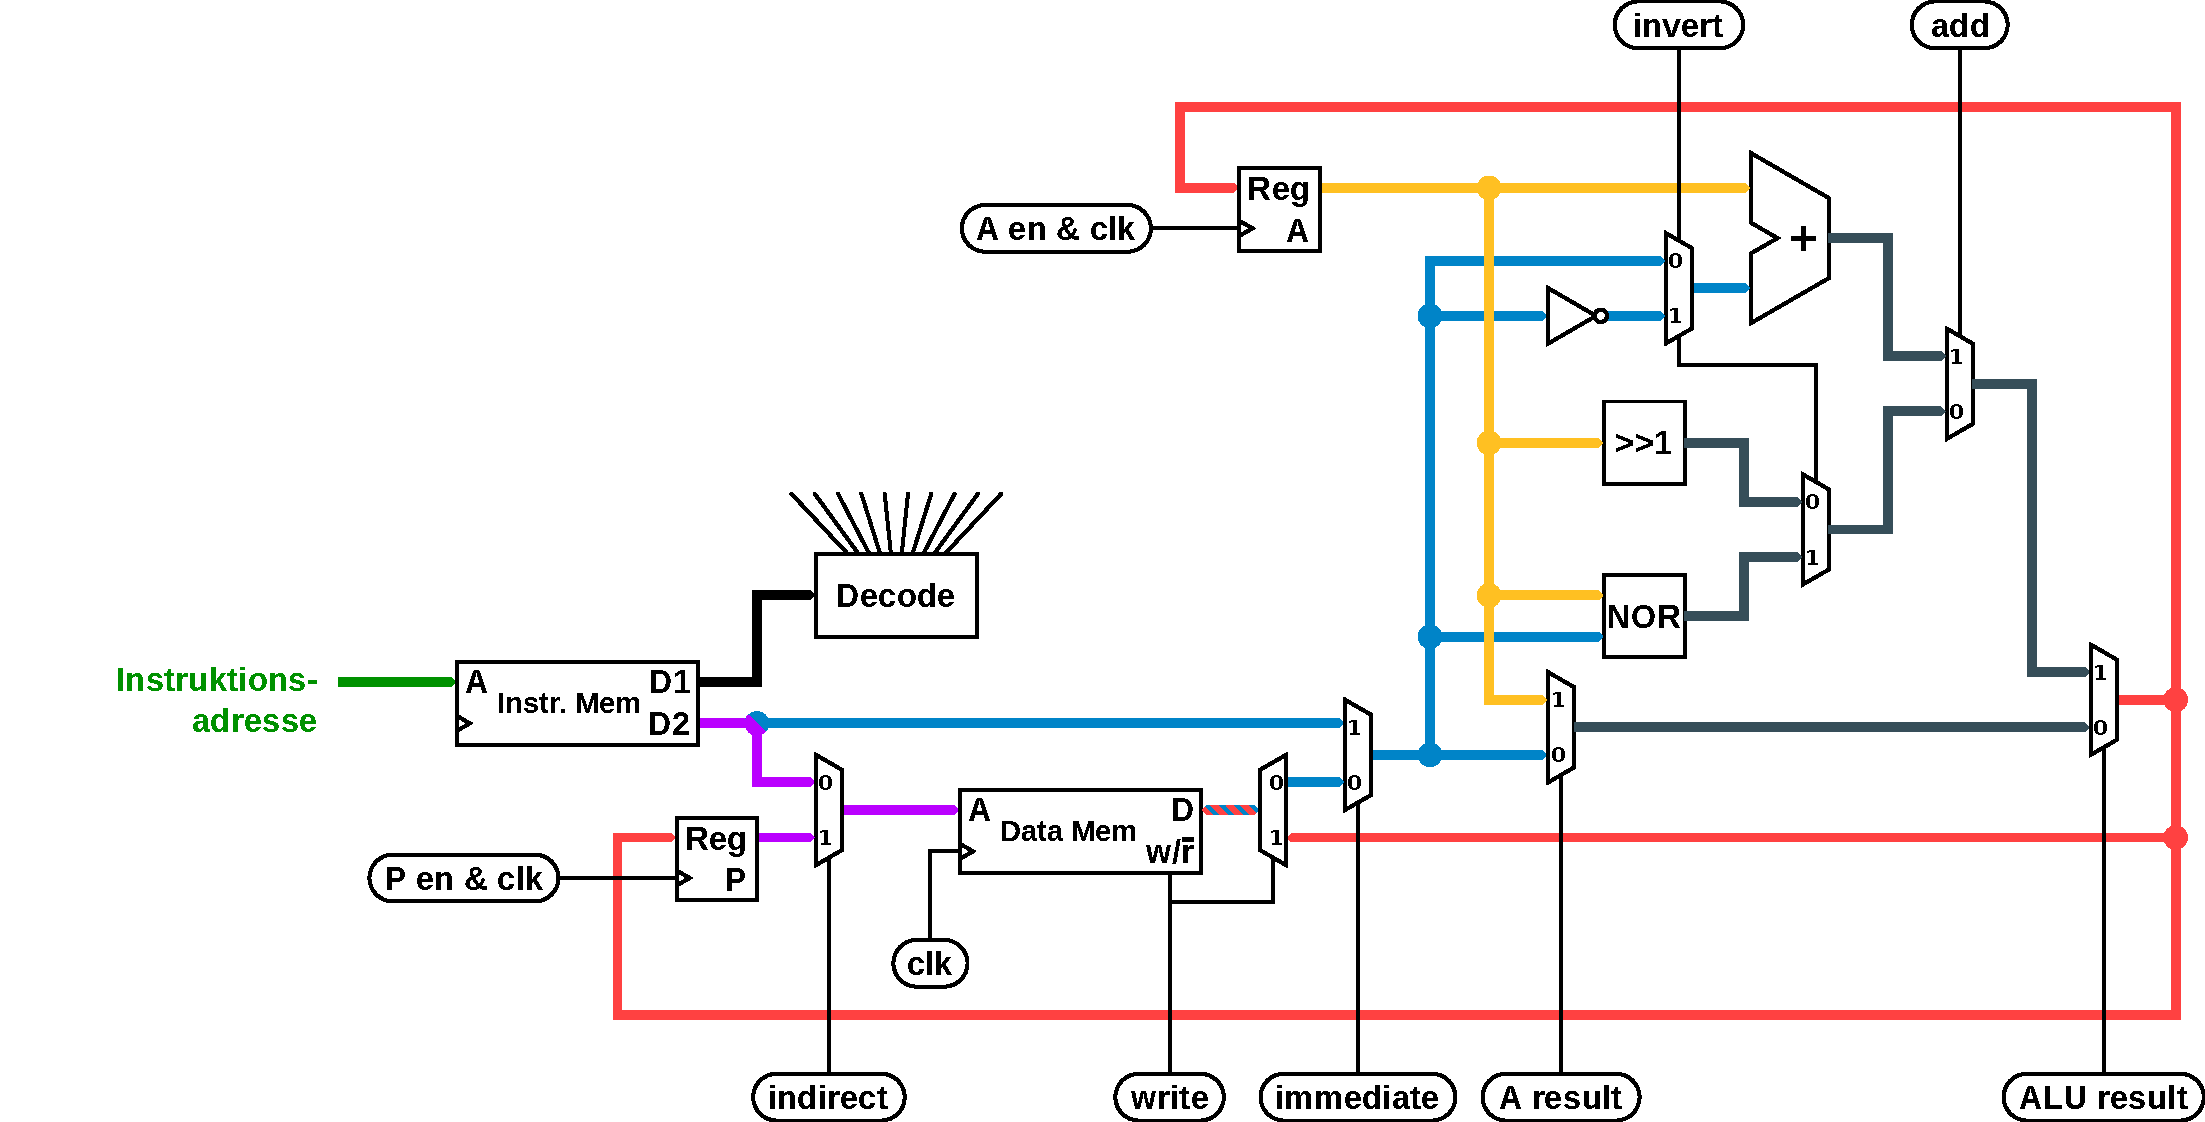
\includegraphics[width=.85\textwidth]{sch-progmem.pdf}
  \end{center}
\end{frame}

\begin{frame}
  \frametitle{Program Counter}

  \strut{}Wenn wir doch nur automatisch zählen könnten~\ldots

  \begin{center}
    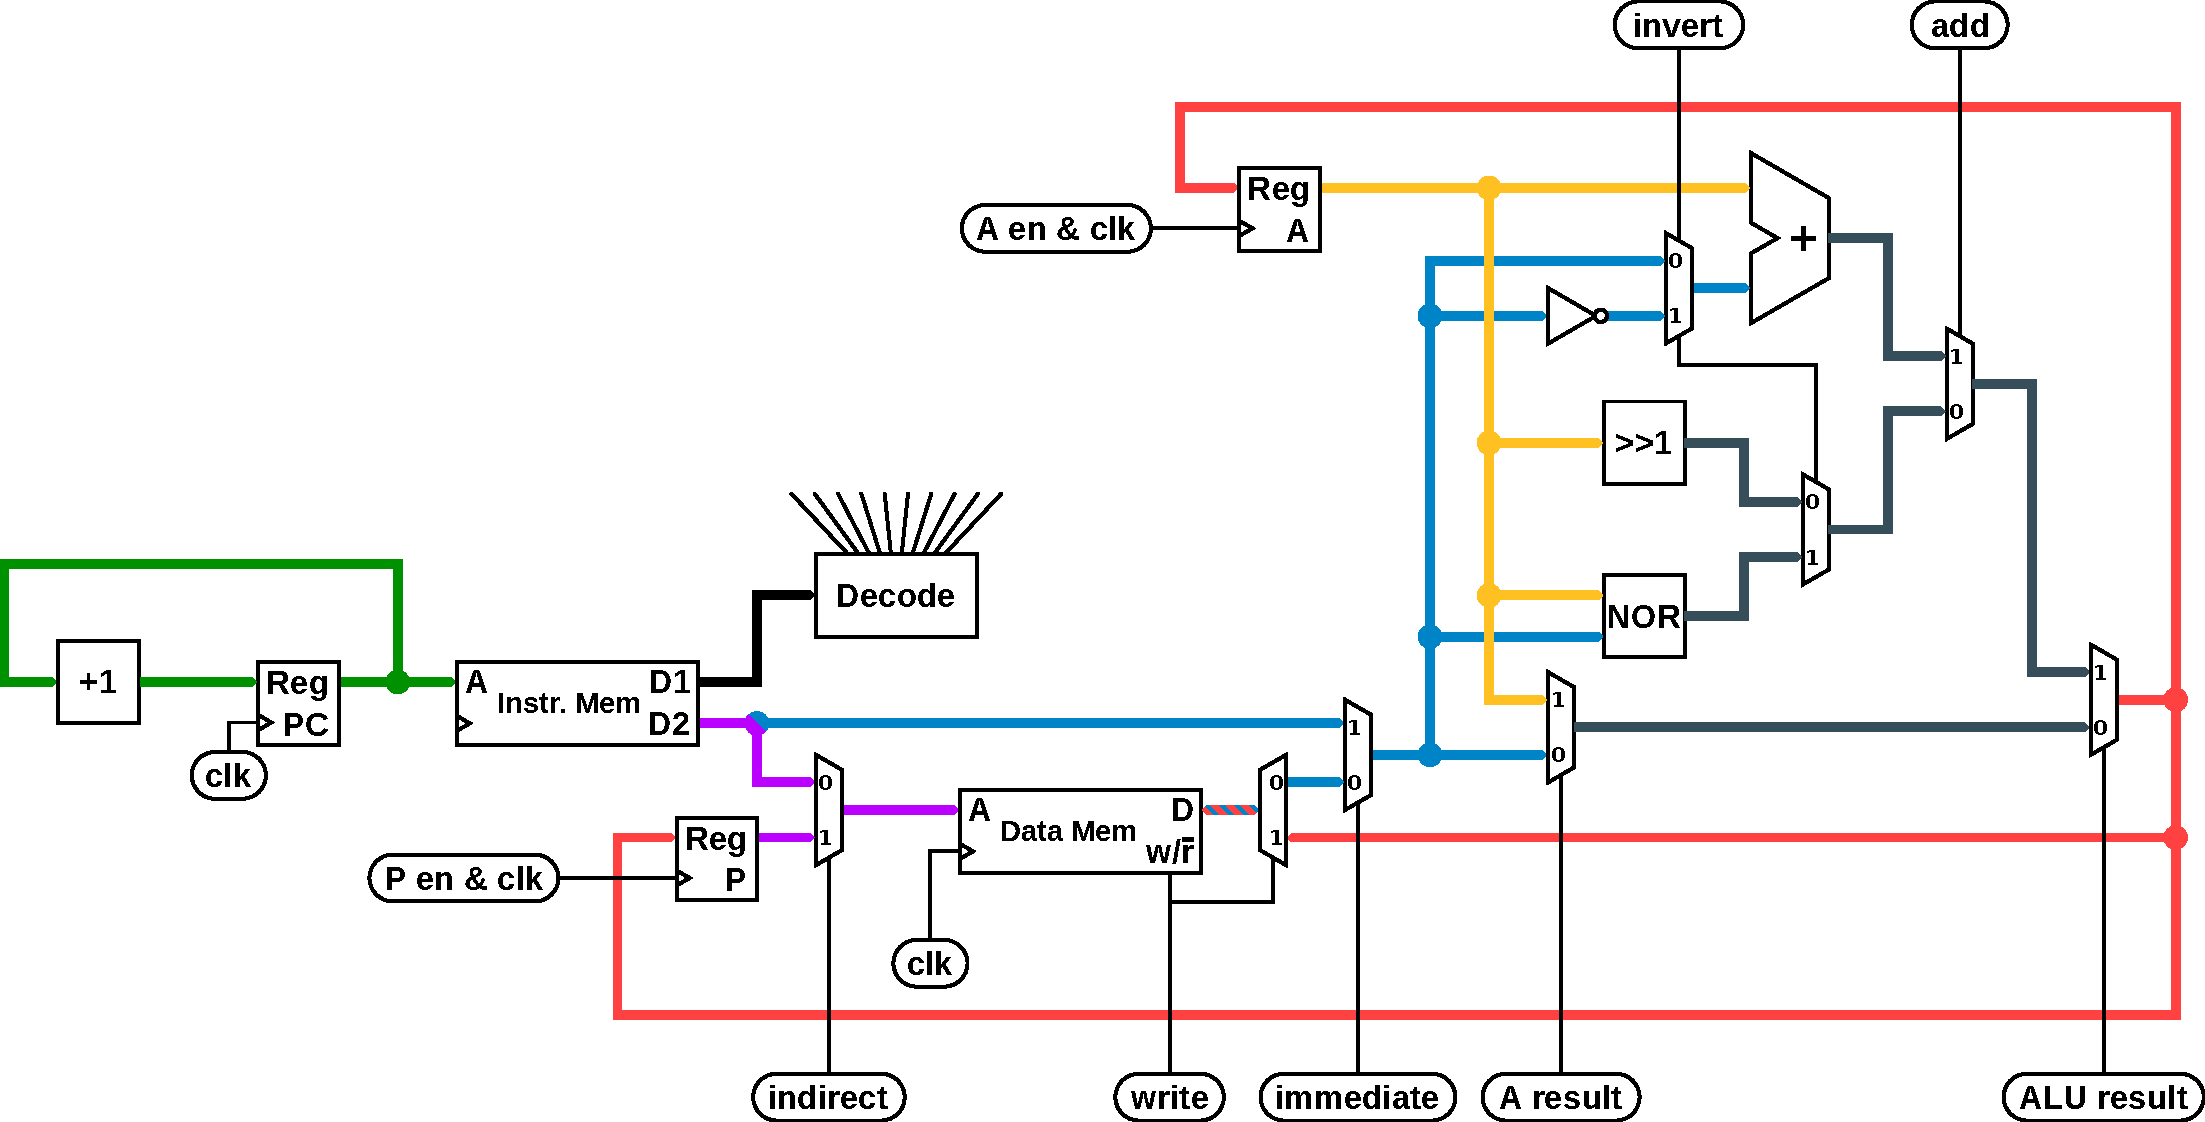
\includegraphics[width=.85\textwidth]{sch-pc.pdf}
  \end{center}
\end{frame}

\begin{frame}
  \frametitle{Sprünge}

  \strut{}Noch ein Mux, die Details sind kompliziert

  \begin{center}
    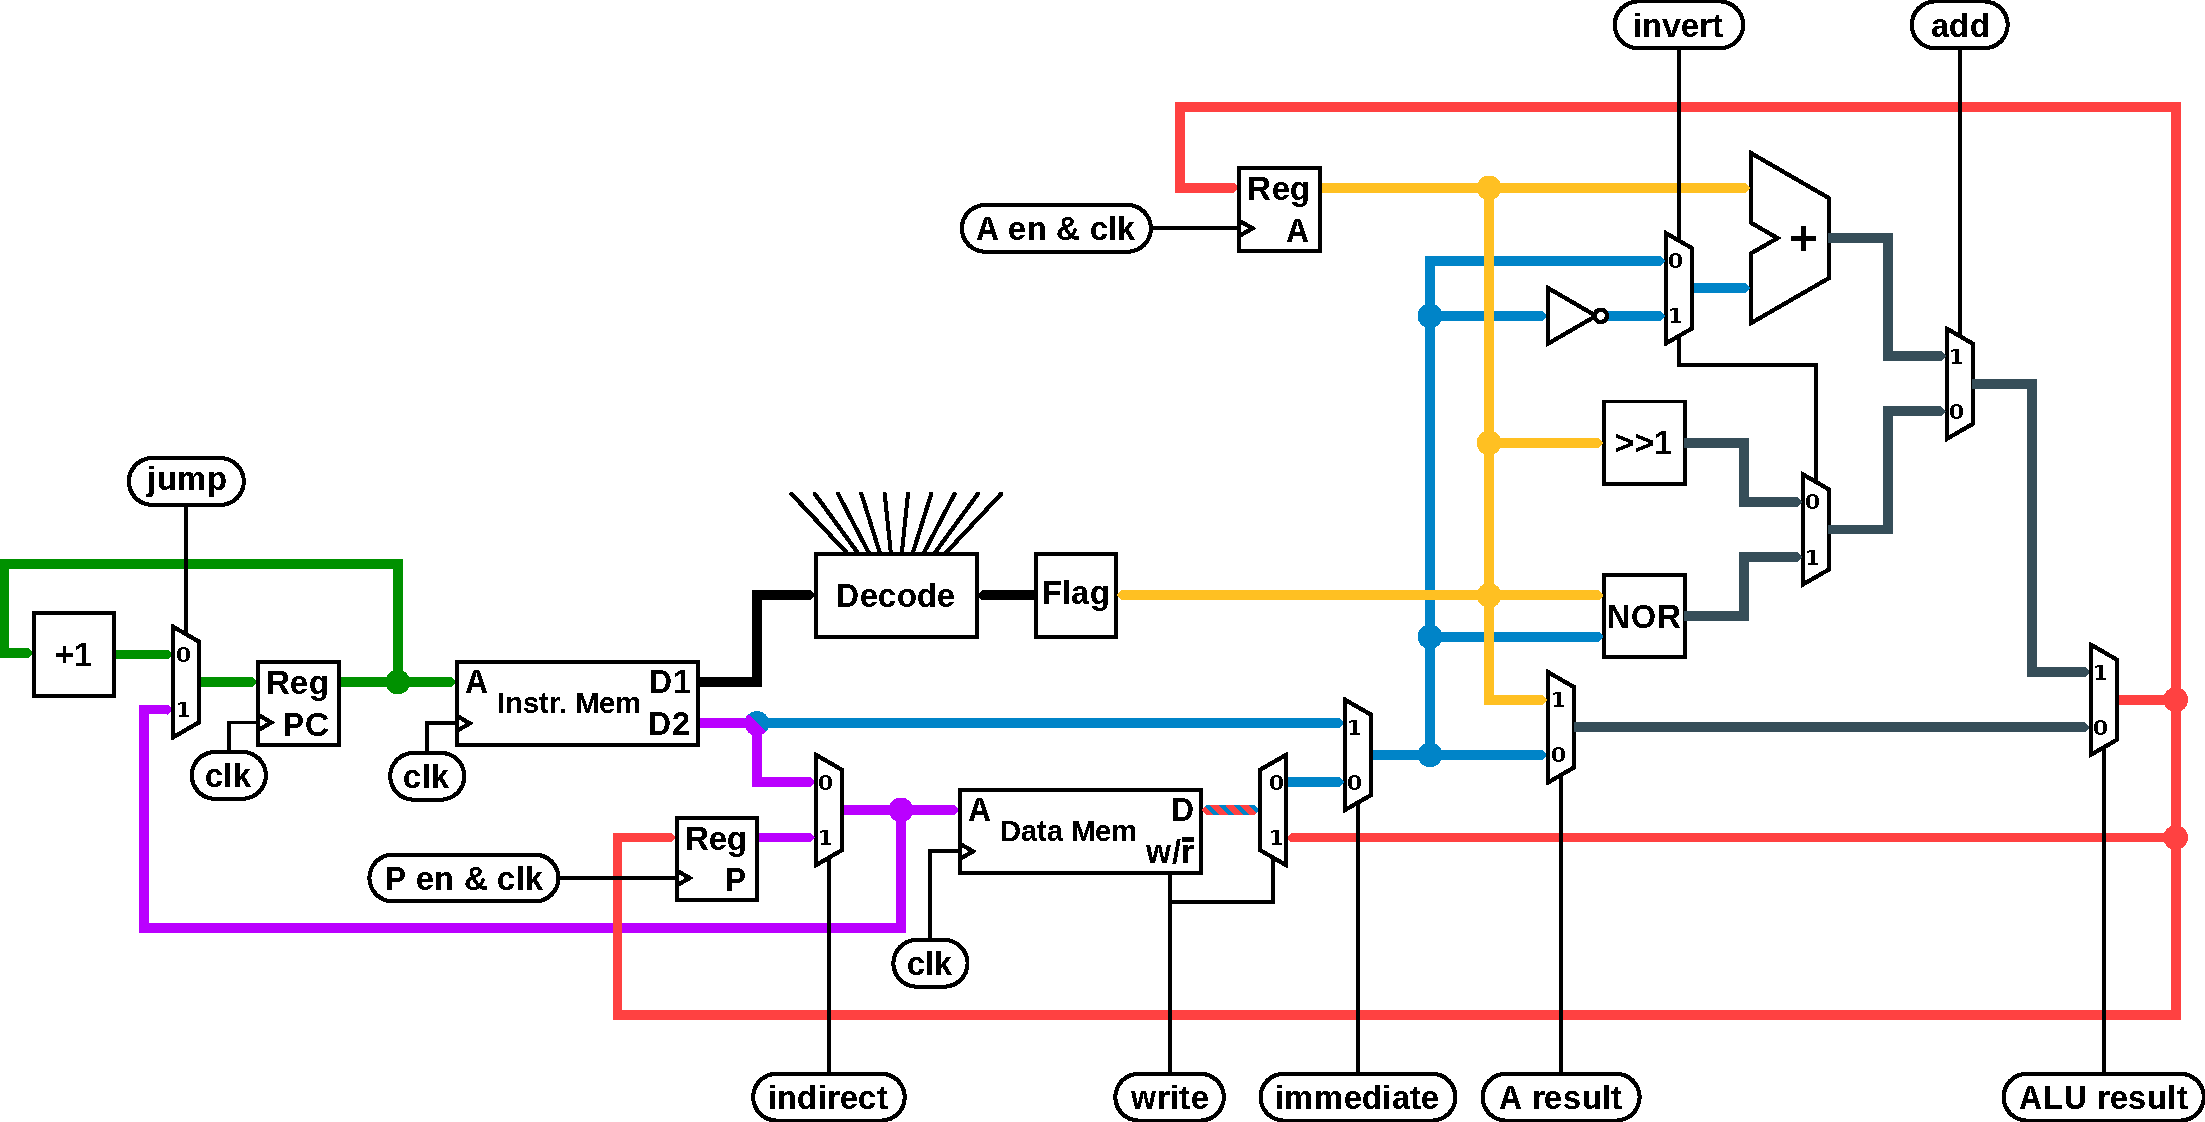
\includegraphics[width=.85\textwidth]{schematic.pdf}
  \end{center}
\end{frame}

\begin{frame}[c]
  \begin{center}
    \Huge{Klick-Klack}
  \end{center}
\end{frame}

\begin{frame}
  \frametitle{Was fehlt?}

  Was wir \enquote{Maschinencode} genannt haben sieht sehr nach \emph{Microcode} aus.
  \begin{itemize}
  \item Viele nutzlose Befehle: \enquote{Addiere \texttt{i} auf Inhalt der Adresse \texttt{i}}, anyone?\\
    \texttt{0x96 i}
  \item 3 Bit für Kombination aus \enquote{A schreiben}, \enquote{P schreiben}, \enquote{Speicher schreiben}\\
    Lieber 3 Bit für Auswahl von einer aus 8 Möglichkeiten!

  \end{itemize}

  \bigskip\pause

  \textbf{Decoding!} Kleinere Assembler-Befehle intern zu Steuersignalen auspacken
\end{frame}

\begin{frame}
  \frametitle{Ihr könnt das auch!}

  und zwar einfacher und besser
  \begin{itemize}
  \item Simulationen/Spiele
  \item Chips statt Relais
  \end{itemize}
\end{frame}

\begin{frame}
  \frametitle{Bildnachweis}
  \tiny
  \begin{description}
    \includecollection{picture-sources}
  \end{description}
\end{frame}

\end{document}